\documentclass[9pt,twocolumn,twoside,lineno]{pnas-new}

\usepackage{lipsum} 
\usepackage[version=4]{mhchem}
\usepackage{siunitx}
\usepackage{mathtools}
\DeclareSIUnit\Molar{M}

%\newcommand{\aucomment}[1]{\textcolor{red}{Author Comment: #1}}
%\newcommand{\inserted}[1]{\textcolor{blue}{#1}}
\newcommand{\aucomment}[1]{}
\newcommand{\inserted}[1]{{#1}}
\newcommand{\dSNPs}{dSNPs~}
\newcommand{\nSNPs}{nSNPs~}
\newcommand{\dSNP}{dSNP~}
\newcommand{\nSNP}{nSNP~}
\newcommand{\hydrochar}{hydrophobicity class}
\newcommand{\chargechar}{charge class}
\newcommand{\cmax}{H_{\rm max}}
\newcommand{\Ht}{H^{\star}}
\newcommand{\het}{\Theta}
\newcommand{\Lw}{L_{\rm w}}
\newcommand{\Lmin}{L_{\rm min}}
\templatetype{pnasresearcharticle} 
\title{Contiguously-hydrophobic sequences are functionally significant throughout the human exome}

\author[a,b]{Ruchi Lohia}
\author[c,1]{Matthew E.B. Hansen}
\author[a,d,1,2]{Grace Brannigan}
\affil[a]{Center for Computational and Integrative Biology, Rutgers University, Camden, NJ, USA}
\affil[b]{Stanley Institute for Cognitive Genomics, Cold Spring Harbor Laboratory, USA}
\affil[c]{Department of Genetics, University of Pennsylvania, Philadelphia, PA, USA}
\affil[d]{Department of Physics, Rutgers University, Camden, NJ, USA}
\leadauthor{Brannigan}

\significancestatement{Proteins rely on the hydrophobic effect to maintain structure and interactions with the environment. Surprisingly, natural selection on amino acid hydrophobicity has not been detected using modern genetic data. Analyses that treat each amino acid separately do not reveal significant results, which we confirm here.  However, because the hydrophobic effect becomes more powerful as more hydrophobic molecules are introduced, we tested whether unbroken stretches of hydrophobic amino acids are under selection. Using genetic variant data from across the human genome, we find evidence that selection increases with the length of the unbroken hydrophobic sequence.  These results could lead to improvements in a wide range of genomic tools as well as insights into protein-aggregation disease etiology and protein evolutionary history.}

\authorcontributions{
 R.L. and G.B. established the blobulation approach. R.L. wrote the blobulation software and performed enrichment analyses.  M.H. ran population-level analyses. R.L., M.H., and G.B. all contributed to design of the study, discussion of results, generation of figures, and writing of the manuscript.}
\authordeclaration{The authors have no competing interests to declare.}
\equalauthors{\textsuperscript{1} Matthew E.B. Hansen and Grace Brannigan contributed equally.}
\correspondingauthor{\textsuperscript{2}To whom correspondence should be addressed. E-mail: grace.brannigan@rutgers.edu}



\begin{document}
\keywords{sequence-function relationship $|$ protein hydrophobicity $|$ single nucleotide polymorphism $|$ population genetics $|$ computational methods} 

\begin{abstract}
\aucomment{Significant insertions of new text are in blue, and comments are in red.}
Hydrophobic interactions have long been established as essential for stabilizing structured proteins as well as drivers of aggregation, but the impact of hydrophobicity on the functional significance of sequence variants has rarely been considered in a genome-wide context. Here we test the role of hydrophobicity on functional impact across 70,000 disease and non-disease associated single nucleotide polymorphisms (SNPs), using enrichment of disease-association as an indicator of functionality. We find that functional impact is uncorrelated with hydrophobicity of the SNP itself, and only weakly correlated with the average local hydrophobicity, but is strongly correlated with both the size and minimum hydrophobicity of the contiguously hydrophobic sequence \inserted{(or ``blob'')} that contains the SNP. Disease-association is found to vary by more than 6-fold as a function of contiguous hydrophobicity parameters, suggesting utility as a prior for identifying causal variation. 
We further find signatures of differential selective constraint on hydrophobic blobs, and that SNPs splitting a long hydrophobic \inserted{blob} or joining two short hydrophobic \inserted{blobs} are particularly likely to be disease-associated. Trends are preserved for both aggregating and non-aggregating proteins, indicating that the role of contiguous hydrophobicity extends well beyond aggregation risk. 
\end{abstract}
\dates{This manuscript was compiled on \today}
\doi{\url{www.pnas.org/cgi/doi/10.1073/pnas.XXXXXXXXXX}}
\maketitle
\thispagestyle{firststyle}
\ifthenelse{\boolean{shortarticle}}{\ifthenelse{\boolean{singlecolumn}}{\abscontentformatted}{\abscontent}}{}
\aucomment{Introduction was reordered, and sentences discussing results were removed for brevity.}
Protein structure is commonly understood to mediate the effects of sequence on function, but single nucleotide polymorphisms (SNPs) can alter function while leaving the protein structure essentially unchanged. For example, intrinsically disordered proteins (IDPs) lack unique structure yet are both essential for many critical biological pathways~\citep {Ward2004,Dyson2005,Uversky2013,Uversky2019,Panchenko2015} and sensitive to sequence~\citep{Weinreb1996, Uverskya,CuanaloContreras2013,Patel2015,Uversky2015,TovoRodrigues2016}. \inserted{A missing framework for sequence modularity and organization presents a conceptual and technical barrier to understanding the underlying mechanisms of sequence dependence, as well as the genetic basis for heritable traits and disease risks.} Structured proteins are clearly modular, but identifying the module boundaries has required explicit knowledge or prediction of secondary structure.  There has been no generic approach for detecting organization when structure is unknown and unpredictable, or non-existent. Here, we propose a general role for contiguous stretches of hydrophobic residues in organizing sequences and determining sequence-sensitivity. 

We showed in a previous study that a long intrinsically disordered protein can retain modularity of tertiary interactions, despite the absence of tertiary structure. Fully-atomistic, explicit-solvent molecular dynamics simulations of the 91-residue disordered prodomain of Brain Derived Neurotrophic Factor (BDNF) revealed a soft network of tertiary contacts between contiguous stretches of hydrophobic residues~\citep{Lohia2019}. In order to distinguish these stretches of hydrophobic residues from any other more traditional segment or domain definition, we follow terminology common to polymer physics and call these stretches  ``blobs''. Blobs may contain secondary structure elements, but are not required to do so. \inserted{These results suggested a more generic framework for interaction-mediated functional modularity, which could be determined directly from sequence. However, the usefulness of this approach had not been tested beyond the single protein in which it was developed. }

Many variant-to-function prediction methods rely on some form of residue characterization of the variant and its local sequence. In addition to physicochemical properties~\citep{Stone2005, Niroula2015, LopezFerrando2017,Hecht2015,Popov2019}
~these may include evolutionary conservation~\citep{Ng2001, Thomas2004, Stone2005,Capriotti2006, Choi2012, Hecht2015, Niroula2015} and structural propensities~\citep{Capriotti2004,Capriotti2005, Parthiban2006, Wainreb2010,Popov2019, Ittisoponpisan2019,Iqbal2020}. Such methods may also rely on known protein structures in order to incorporate properties such as local secondary structure and solvent accessibility~\citep{Iqbal2020}. Fewer than 35\% of human protein coding genes have structures deposited in the protein data bank~\citep{Prlic2016}, and complete structures have been experimentally solved for a tiny fraction of known proteins~\citep{Rose2016,Mir2017}.   

In the absence of structural information, physicochemical properties like hydrophobicity can still be determined from sequence, but the properties of individual residues are not predictive. Most attempts at incorporating the local sequence have used a fixed-width sliding window centered around the SNP, which neglects the intrinsic modularity of protein sequences and may contribute to the relative weakness of these approaches. For example, if the mutated residue is near the module boundary, the mutation-centered window will partially overlap a module that does not contain the SNP. We propose here that the blob surrounding a residue provides a natural and sequence-informed definition for the local sequence context.  Furthermore, due to the cooperativity of the hydrophobic effect~\citep{Jiang2017} and the tendency for hydrophobic residues to be buried~\citep{Lins2003}, we hypothesized that hydrophobic blobs (``h-blobs'') would form interaction-rich and mutation-sensitive clusters across a generic proteome. 

In the present work, we detect h-blobs across the human proteome and characterize their structural properties and functional impact. \inserted{We calculate the distribution of secondary structures for residues inside and outside h-blobs, and use solvent-accessibility calculations to test our hypothesis that h-blobs represent buried regions of solvated proteins. Our analysis of function uses disease-association as a proxy for functional impact.} We test for enrichment of disease-associated SNPs as a function of hydrophobic blob length, residue hydrophobicity, and average hydrophobicity of a window centered around the SNP. We complement these results using population frequencies to test for signatures of selective constraint in h-blobs. \inserted{Furthermore, we consider functional impact within multiple special cases, including transmembrane regions, aggregating proteins, and SNPs that split or merge blobs or change specific blob properties.} In sum, we shall present several signatures consistent with the hypothesis that proteins are partly organized around domains of contiguous hydrophobicity, and demonstrate that we can roughly delineate such regions from sequence alone. 

\section*{Results}

\subsection*{Regions of contiguous hydrophobicity are enriched for $\beta$-strands and buried residues}
\label{section:1}

\begin{figure}
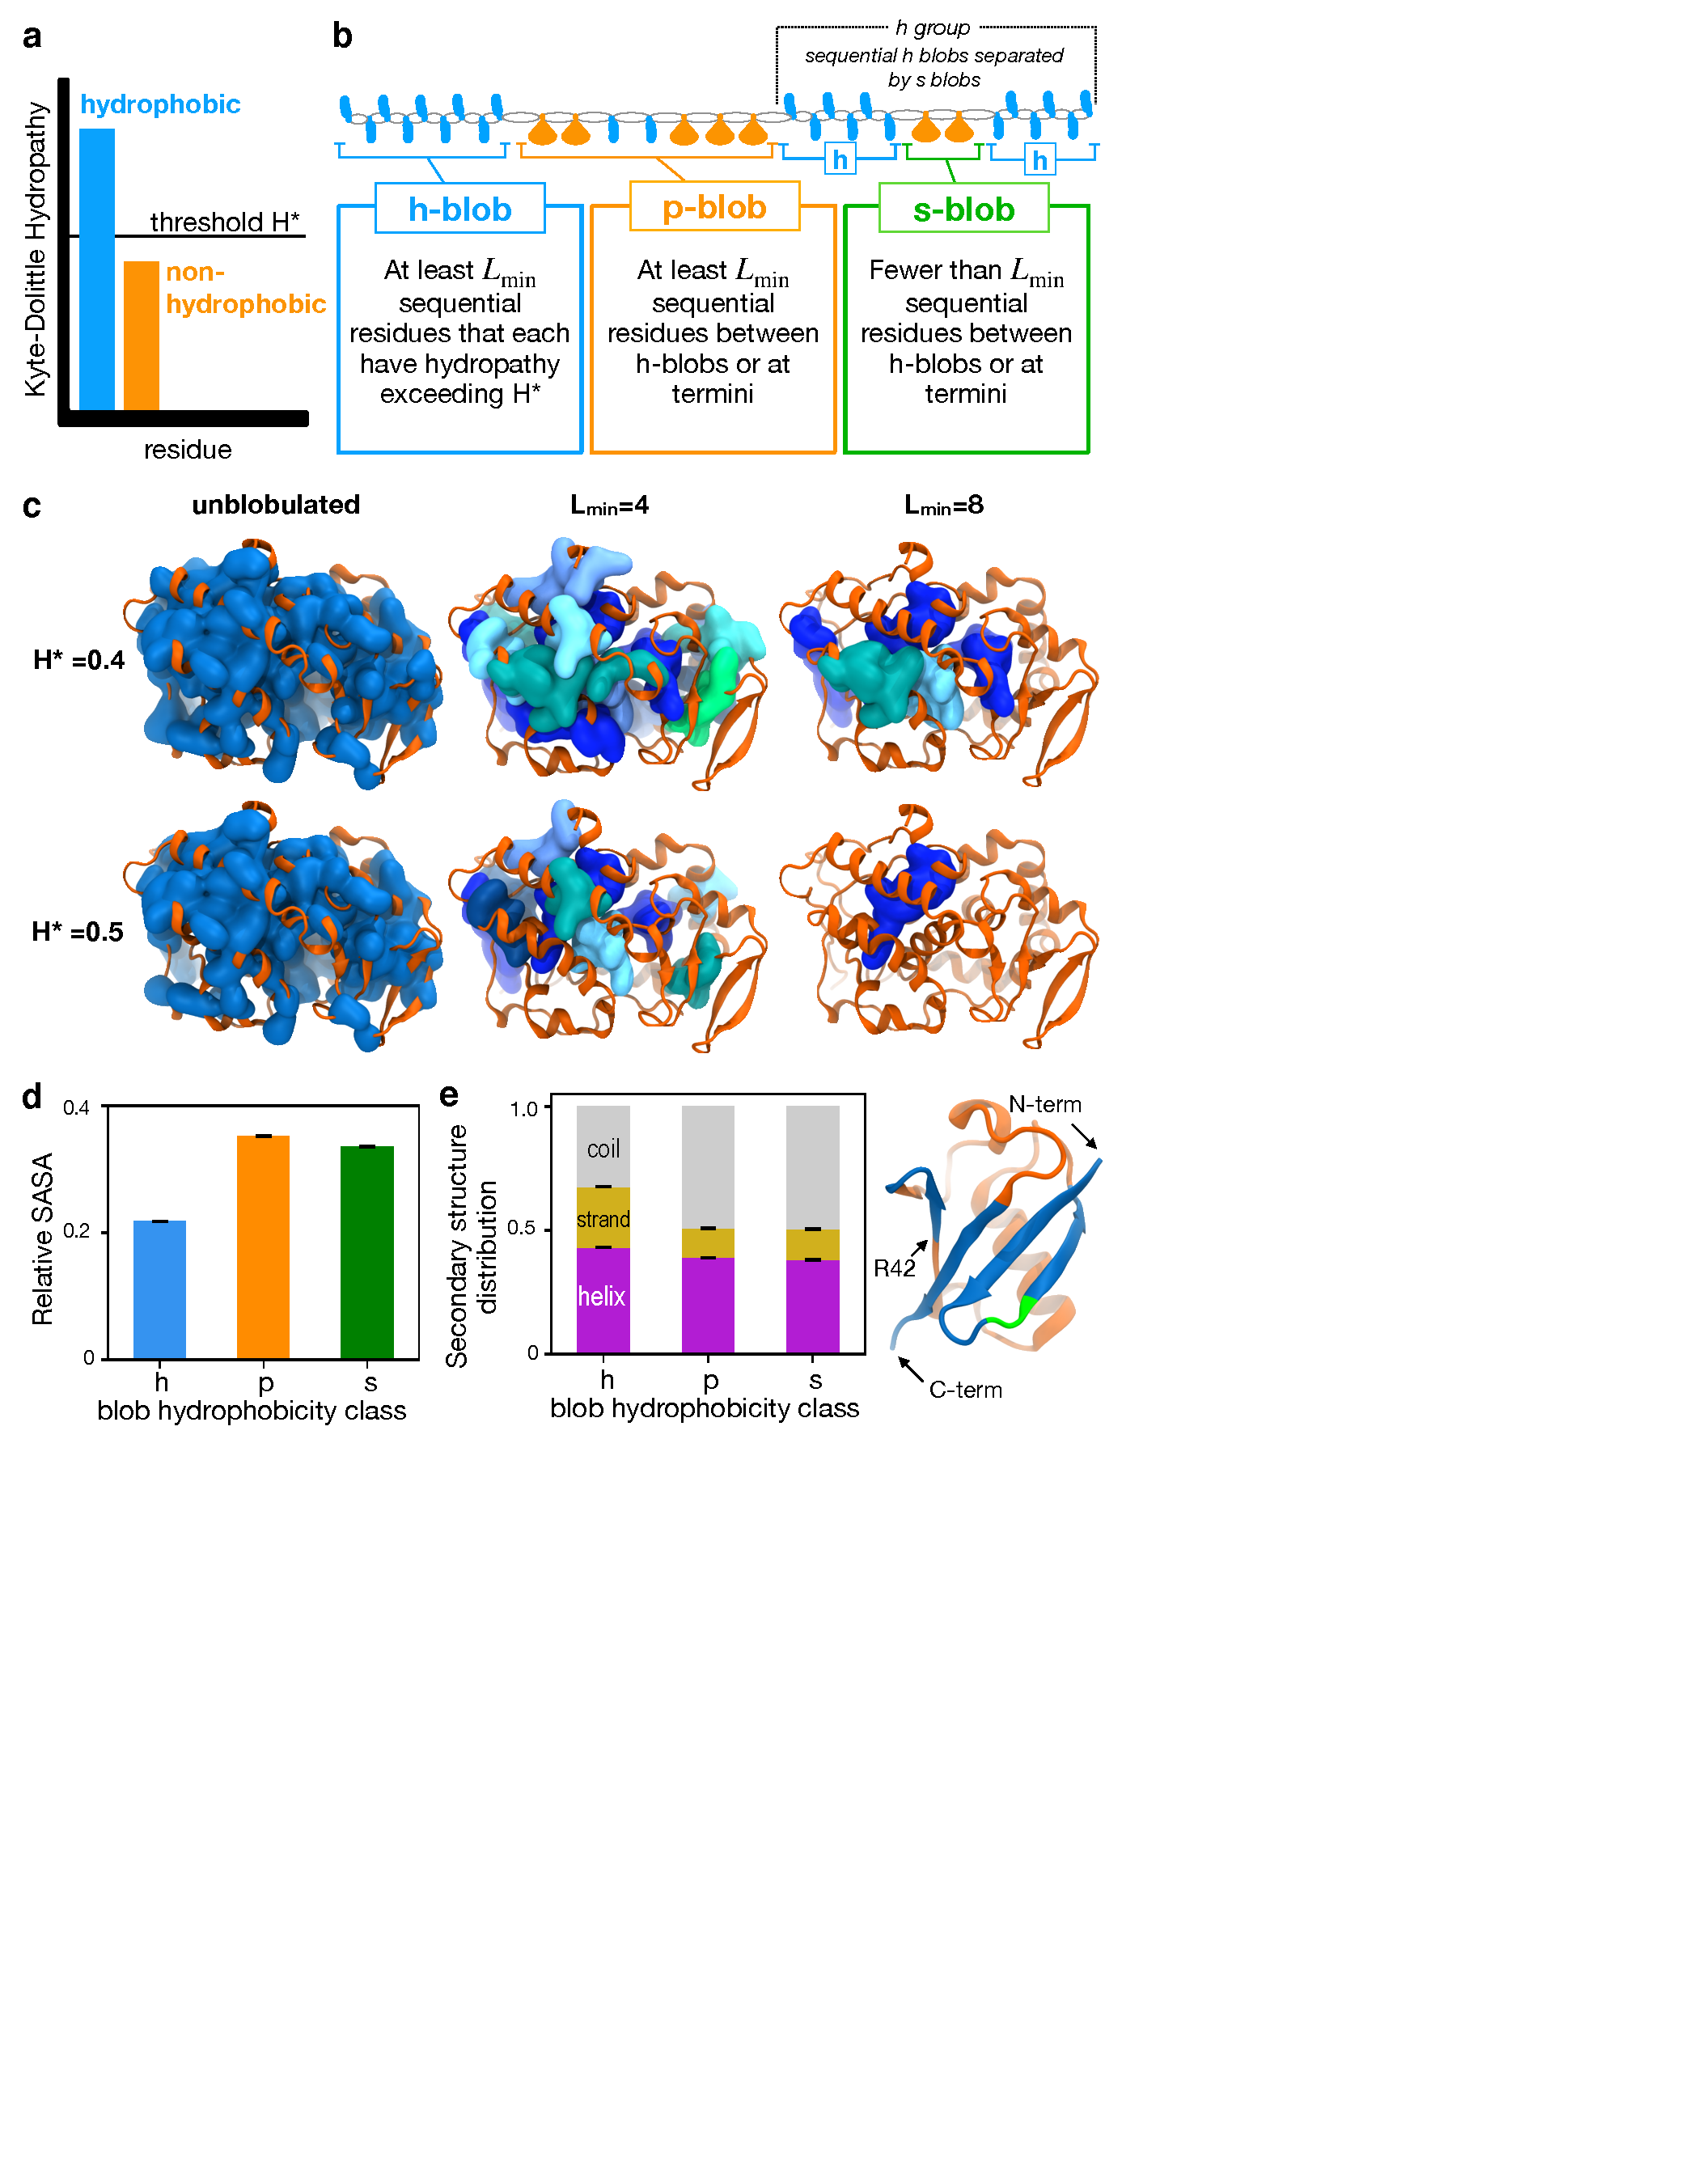
\includegraphics[width=0.5\textwidth]{fig1.pdf}
\caption{{\bf Whole-sequence blobulation algorithm for segmentation of proteins.} \aucomment{Panels 1a and 1b replace the previous figure 1. Panels c-e are entirely new.} a) First, the sequence is digitized: residues are classified as hydrophobic or non-hydrophobic depending on whether they have a Kyte-Dolittle \cite{Kyte1982} hydropathy falling above or below the user-provided threshold $\Ht$, respectively. b) The clustering step acts on the digitized sequence, which is illustrated here as a cartoon: residues above and below the $\Ht$ threshold are shown as blue ovals and orange fans respectively. The clustering step scans the digitized sequence according to the indicated criteria, first detecting h-blobs, then p-blobs, and finally s-blobs. $\Lmin$ is the user-provided minimum blob size. The blobulation outcome for this particular chain would be valid for $2<\Lmin<6$. The software and a web-interface are freely available as described in {\em Materials and Methods}. c) Cytochrome C peroxidase (2CYP~\cite{Finzel1984}) shown for two different digitization thresholds $\Ht$ (rows), and three different clustering criteria (columns), including no clustering (left ``unblobulated'' column) or two different values of $\Lmin$ (middle and right column, respectively).  The blue surface of the unblobulated sequence depicts canonical hydrophobic residues; the $\Ht=0.4$ row also includes Serine and Threonine, which have Kyte-Dolittle hydropathy scores of 0.41 and 0.42 respectively. H-blobs in the middle and right columns are colored by arbitrarily varying shades of blue to distinguish individual blobs. d) Relative solvent-accessible surface area (SASA) for non-transmembrane blobs in the Protein Data Bank (PDB), categorized by blob hydrophobicity class. e) Left: Distribution of secondary structures for sequences with structures in the PDB, categorized by blob hydrophobicity class. Right: Blobulated ubiquitin (PDBID 5GO7~\cite{Gao2016}), colored by blob hydrophobicity class, as in B. In both panels d and e, the blobulation algorithm uses $\Lmin=4$ and $\Ht=0.4$; error bars are standard errors ($n>500,000$ for h- and p-blobs, $n>50,000$ for s- blobs). See {\em Materials and Methods} for details.}
\label{cartoon} 
\end{figure}

\aucomment{This subsection is entirely new.}
\inserted{The blobulation algorithm, first presented in Ref. \cite{Lohia2019}, is a method for tunable segmentation or edge detection in protein sequences based on hydrophobicity. The original ``whole-sequence'' blobulation algorithm digitizes the sequence and then clusters it. In the preliminary digitization step (Fig. \ref{cartoon}A), each residue is classified as hydrophobic or non-hydrophobic, depending on whether the Kyte-Dolittle hydropathy score~\cite{Kyte1982} is above or below the hydrophobicity threshold $\Ht$. In the main clustering step (Fig. \ref{cartoon}B),  the algorithm scans the given amino acid sequence to identify stretches of at least $\Lmin$ sequential residues that were classified as hydrophobic during digitization. These stretches are called hydrophobic blobs or ``h-blobs''. }

\inserted{The residues that are not assigned to h-blobs will contain a mix of non-hydrophobic residues and isolated hydrophobic residues, in stretches that either link h-blobs or terminate the sequence: short stretches that contain fewer than $\Lmin$ residues are classified as separator or ``s-blobs'', while long stretches with at least $\Lmin$ residues are classified as polar or ``p-blobs.'' The blobs can then be characterized based on any collective property of the blob sequence; the h, p, and s designation also constitute the primary blob characterization termed the ``\hydrochar''. In Ref. \cite{Lohia2019} we also introduced a higher order classification: adjacent h-blobs that were separated only by the short s-blobs were called ``h-groups''. We include this designation in Fig. \ref{cartoon}B for completeness but do not explicitly consider h-groups in this paper. However, h-groups \emph{are} captured implicitly by variation of the $\Ht$ threshold; the long h-blobs that are detected at low $\Ht$ would be classified as h-groups at high $\Ht$.} 

\inserted{The blobulation algorithm can be used in multiple ways, and we apply it in three slightly different ways within this study. In the original ``whole sequence'' version just described, the entire sequence is unambiguously and completely decomposed into h-, p-, and s-blobs using two fixed parameters $\{\Ht,\Lmin\}$ provided by the user.  In this section we will continue to use this approach, because the analysis considers whole proteins. Alternatively, we can fix one residue and one parameter, and calculate or optimize the second parameter. In subsequent sections we will use two such variations (``unconstrained length'' and ``unconstrained threshold'') for analyzing the blob properties surrounding specific sets of SNPs. Both approaches are described further at first use. }

\inserted{We find that nearly half of the residues in the proteome meet our original~\cite{Lohia2019} relaxed criteria for h-blobs, which includes short, moderately hydrophobic sequences. More specifically, using $\Lmin=4$ and $\Ht=0.4$, the residues in the Universal Protein Resource (UniProt) database~\cite{Bateman2021} (N = 6,459 proteins) are distributed as follows: 45\% in h-blobs, 52\% in p-blobs, and 3\% in s-blobs. Stricter criteria can be used to isolate the long, highly hydrophobic blobs that cover less than 10\% of the proteome: using $\Ht=0.5$ and $\Lmin=8$, the distribution is 7\% in h-blobs, 93\% in p-blobs, and $<1$\% in s-blobs. The effect of varying these two parameters is shown for cytochrome C peroxidase in Fig. \ref{cartoon}C; as the criteria is made more restrictive, the algorithm isolates one long and very hydrophobic blob at the core of the protein.}

\inserted{To test the hypothesis that h-blobs would be buried in globular, structured proteins, we calculated the relative solvent-accessibility surface area (SASA) for each blob type, determined using structures in the Protein Data Bank (PDB) (excluding transmembrane domains). Relaxed criteria ($\Lmin=4, \Ht=0.4$) were used for this calculation to maximize the amount of available data and to keep the analysis conservative (Dataset S1).  These calculations (Fig. \ref{cartoon}D) confirmed that residues in h-blobs have a substantially lower SASA (0.21) than p-blobs (0.35) or s-blobs (0.33); standard error for all three quantities is less than 0.001. Together, these results suggest that h-blobs condense into buried clusters that are rich in intra- or inter-protein interactions. As illustrated in Fig. \ref{cartoon}C, we expect this difference to be even larger for h-blobs that meet stricter criteria.}

\inserted{The overlap between blob \hydrochar{} and secondary structure was measured by blobulating all unique proteins in the PDB and tabulating the fraction of residues occurring in helices ($\alpha$, 3-10, $\pi$), strand ($\beta$-bridge or extended $\beta$ strand), or coil for each blob type (Dataset S2). 
As shown in Fig. \ref{cartoon}E, all blob types contain a comparable fraction of helices, although the fraction in h-blobs is slightly greater than in non h-blobs. We do not expect contiguous hydrophobicity to be particularly correlated with helical structure (with the exception of transmembrane helices): helices frequently have multiple faces with differential solvent accessibility, and the sequence needs to cycle through residues that are appropriate for each face. H-blobs, however, are about twice as likely to contain strands as non h-blobs (Fig. \ref{cartoon}E). $\beta$-strands are secondary structure elements, but they are also indicators of tertiary interactions, since $\beta$-strands will have a pairing $\beta$-strand. These results are consistent with our first application of blobulation to simulated conformations of the long disordered pro region of BDNF~\cite{Lohia2019}, which revealed a network of soft tertiary interactions mediated through pairing of $\beta$ strands in h-blobs. }

\inserted{As an example, Fig. \ref{cartoon}E also shows the blob assignments for the ubiquitin sequence mapped onto its structure. The N-terminal $\beta$-hairpin is assigned to two h-blobs, separated by an s-blob that is adjacent to the turn. The C-terminal $\beta$-strand is also assigned to an h-blob, capped by an s-blob at the terminus. Finally, the Pro37-Ala46 $\beta$-strand is a p-blob from Pro37 to Arg42 and then switches to an h-blob as it crosses into the h-blob rich part of the protein. That h-blob continues until the chain bends back toward the other p-blobs. This example suggests that while blob boundaries can align with secondary structure elements, they are more fundamentally correlated with the location of the blob within the three-dimensional protein structure. }

\subsection*{Average local hydrophobicity is a weak indicator of disease-association}
\aucomment{In the previous version, this subsection and the next were joined. They were split and content was reordered to accommodate the new information on transmembrane domains}
In order to test whether the residue hydrophobicity is {\em prima facie} correlated with functional impact, we calculated the enrichment of disease-associated missense SNPs (``dSNPs'') as a function of hydrophobicity of the reference allele. Throughout this paper, unless otherwise noted, \dSNPs are tested for enrichment relative to the expectation set by missense SNPs that are not disease-associated (``nSNPs''). For example, the phrase ``\dSNPs are enriched in blobs of type X'' means that the proportion of \dSNPs found in blobs of type X is larger than the proportion of \nSNPs found in blobs of type X. As shown in Fig. \ref{blob_vs_window}B, we did not detect any significant correlation (Pearson's r=0.02, n=17) between lone SNP hydrophobicity and dSNP enrichment, meaning that the hydrophobicity of a residue considered in isolation does not show this particular signature of functionality.

The effect of average local hydrophobicity on the enrichment of dSNPs was calculated using moving windows of length $\Lw$ centered around each SNP. 
While there is no ``standard'' window size, most SNP prediction programs use a window size in the range of 1-21 residues~\citep{Teng2010, Capriotti2006, Capriotti2017, Hecht2015}. The window size is chosen to balance concerns that small window sizes may not accurately capture the ``local'' sequence~\citep{Chen2006, Schlessinger2005, Sander2006} whereas long window sizes can decrease signal to noise ratio~\citep{Park2007}.  Here we computed the mean window hydrophobicity $\bar{H}_i$ for all SNPs $i$ in our SNP dataset, while also varying $\Lw$. Fig. \ref{blob_vs_window}C shows the enrichment of \dSNPs for which $\bar{H}_i > \Ht$, for the range of moving window widths $\Lw=1-99$. As is evident in Fig. \ref{blob_vs_window}C, the enrichment of \dSNPs is relatively insensitive to the window size for the regime where $\Lw \ge 6$ and $\Ht \le 0.65$. The total count of \nSNPs in each bin is shown in Fig ~\ref{blob_vs_window}G, and was similarly insensitive to window size for larger thresholds. These results suggest that distant residues introduce noise that averages out in a proteome-wide analysis, but their inclusion in the window would still reduce precision for any individual SNP. 

Surprisingly, we detect a narrow band of \dSNP depletion for windows with a high average hydrophobicity (the red signal for $\Ht\ge 0.65$ in Fig. \ref{blob_vs_window}C). This signal is due to only a handful of SNPs (see the counts in Fig. \ref{blob_vs_window}G), but we observe a similar pattern using the blobulation algorithm, and we discuss its origins in the next sections.

\begin{figure*}
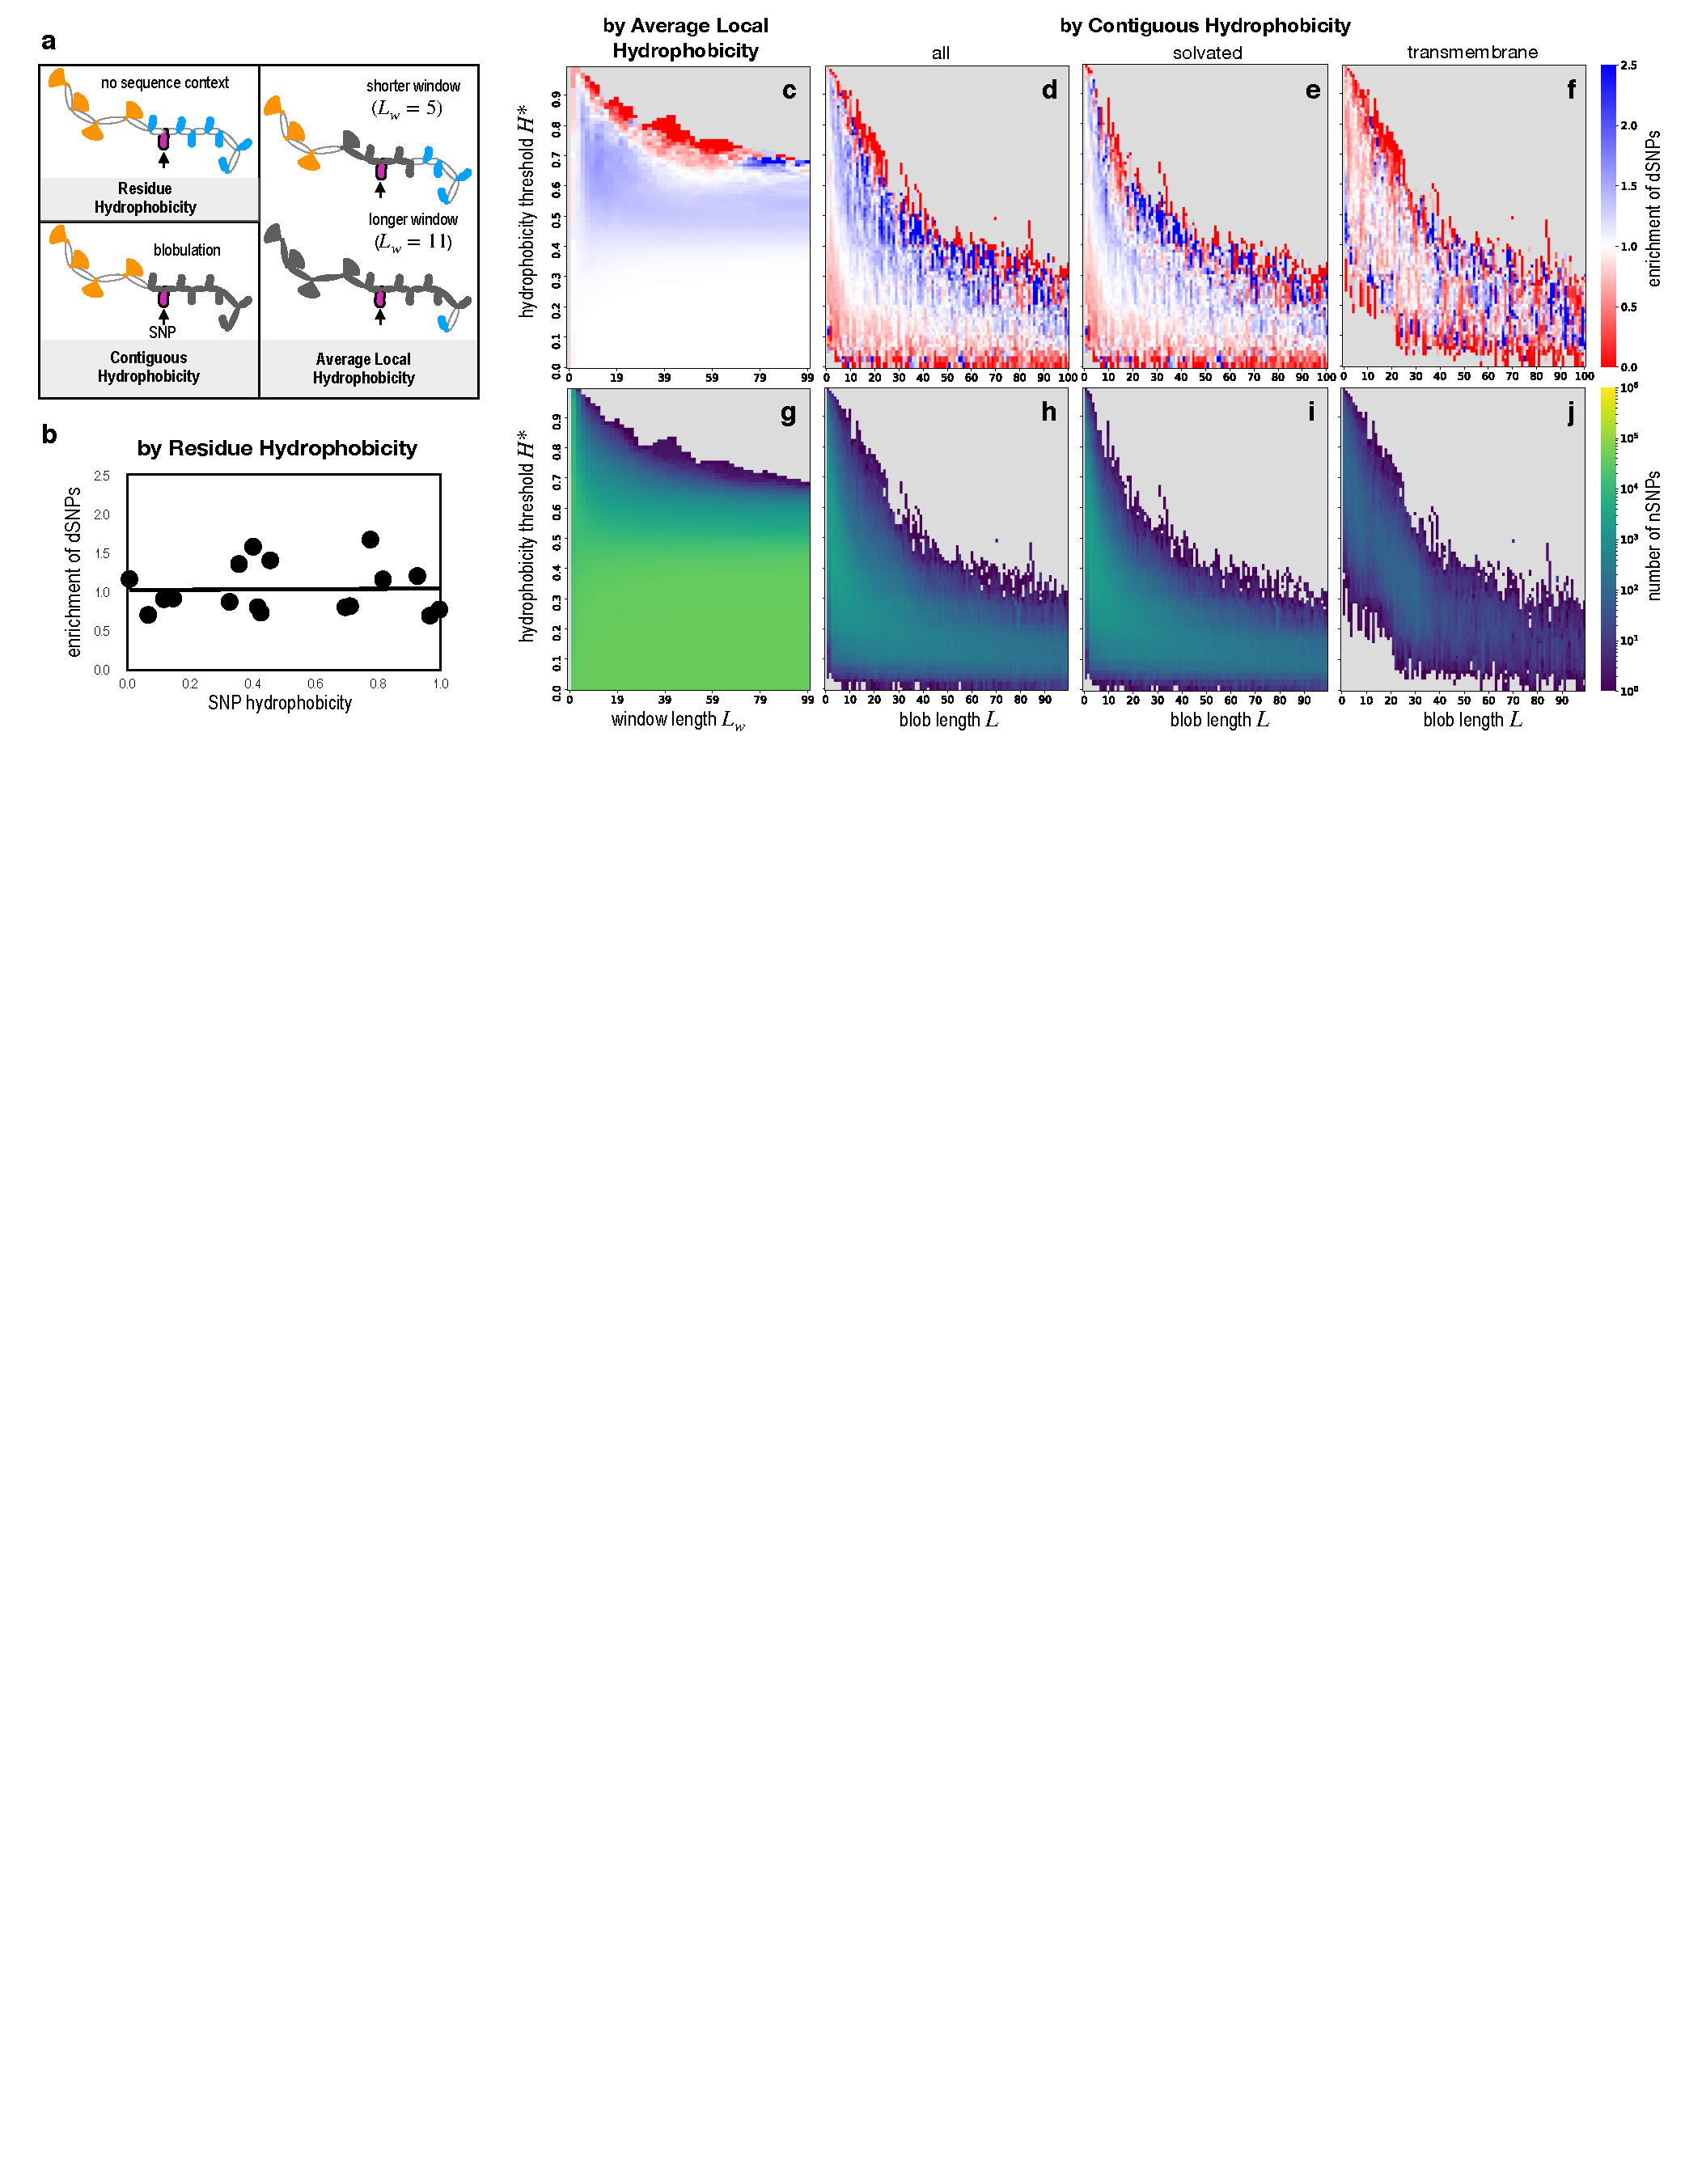
\includegraphics[scale=1,width=\textwidth,trim={0 0cm 0 0cm},clip]{fig2.pdf}
\caption{{\bf Effect of segmentation approach, length,  hydrophobicity threshold, and environment on calculated enrichment of \dSNPs in hydrophobic segments.} a) Illustration of three measures of SNP hydrophobicity (residue, contiguous, and average local) for the indicated SNP, found within a hypothetical peptide chain composed of residues classified as hydrophobic (blue ovals) or non-hydrophobic (orange fans) for a given $\Ht$, as in Fig. \ref{cartoon}B. Unconstrained-length blobulation determines the local sequence (shaded in gray) by detecting contiguous hydrophobic residues, which together form an h-blob of length $L$; the moving window approach determines the local sequence using a fixed number $L_w$ of residues centered around the SNP. b) Enrichment of disease-associate SNPs (dSNPs) relative to non disease-associated SNPs (nSNPs) as a function of hydrophobicity of the reference allele, with line of best fit. No trend or significant correlation is observed (Pearson's r=0.02, p=0.94, n=17). (c-f) Enrichment of \dSNPs in hydrophobic segments, as a function of segment length and threshold, for (c) fixed-length hydrophobic windows of length $L_w$ in which the average hydrophobicity is above $\Ht$, or (d-f) h-blobs of length $L$, calculated with the threshold $\Ht$ for (d) all SNPs, \inserted{(e) those outside of transmembrane domains or (f) those in transmembrane domains.}
g-j) The total number of nSNPs per bin for the corresponding enrichment heatmaps in the row above, e.g. i) shows the nSNP counts for the enrichments in e). 
Each panel (c-j) is colored according to the scale at the right end of the row, and bins with no data are colored gray. \aucomment{Panels e,f,i, and j are new. Annotations were added to the other panels.}}
\label{blob_vs_window} 
\end{figure*}

\subsection*{Contiguous hydrophobicity is a strong indicator of disease-association}

The use of a fixed-width window neglects the inherent dispersion in the size of protein modules, which are captured using blobulation (Fig. ~\ref{blob_vs_window}A). To quantify the blob properties for each SNP, we used a blobulation variant we call ``unconstrained length'' blobulation, which fixes the threshold $\Ht$ and a reference residue $i$ but imposes no minimum blob length. This approach first tests whether the hydropathy score for residue $i$ exceeds $\Ht$, and if so, it calculates the exact length $L$ of the h-blob that contains residue $i$. ``Unconstrained length'' blobulation is formally equivalent to ``whole-sequence'' blobulation with $\Lmin=1$, but is more efficient since we are only analyzing the relevant part of the sequence. 

Specifically, we applied unconstrained-length blobulation to each SNP in the dataset (using the reference allele) and a given hydrophobicity threshold $\Ht$, and then determined $L$.  We repeated this calculation for a series of $\Ht$ values, and for dSNPs and nSNPs separately (Dataset S3), and then tabulated the proportion of dSNPs and nSNPs in each $(\Ht,L)$ bin (Dataset S4). The resulting enrichment of \dSNPs as a function of blob length $L$ and threshold $\Ht$ is shown in Fig. \ref{blob_vs_window}D, and the total number of \nSNPs per bin shown in Fig. \ref{blob_vs_window}H.
We observe a consistent relationship between hydrophobicity of the local blob and \dSNP enrichment.  \dSNPs are depleted in weakly hydrophobic blobs, neutral for moderately hydrophobic blobs, and become more enriched as the blob gets longer and/or satisfies a stricter hydrophobicity threshold. The trend is steadily monotonic, which supports the hypothesis that hydrophobic blobs constitute identifiable functional elements.

We do find an exception to the trend at the plot boundary: blobs that satisfied the very strictest criteria were depleted in dSNPs, consistent with the results using the moving window analysis. The depletion signal persisted even when bins with very few blobs were removed. In the next section, we consider two potential reasons for this depletion: either \dSNPs in these blobs are so deleterious that they are selected out of the population, or some subset of \nSNPs are functional and under balancing selection or relaxed constraint. In addition to a consistent trend, the analysis returns a large spread in enrichment/depletion values:  3.2\% of the bins in Fig. ~\ref{blob_vs_window}D are significantly depleted below 0.5, while 13\% have a significant enrichment of greater than 1.5, and 3.5\% have a significant enrichment greater than 3 (significance based on Binomial test, $P<10^{-3}$, see {\em Materials and Methods}). This range indicates that hydrophobicity-based sequence segmentation could be particularly useful for assessing the riskiness of SNPs located in long or very hydrophobic sequences. To this end, the numerical enrichment values for each bin are provided in Dataset S4.

\inserted{Transmembrane helices will intrinsically require contiguous residues that are at least moderately hydrophobic (with the exception of pore-lining helices) and it seemed possible that our results were dominated by the distinctive properties of such transmembrane domains. We further decomposed the data into contributions from SNPs that are not in transmembrane domains (Fig. \ref{blob_vs_window}E) and those that are (Fig. \ref{blob_vs_window}F). The counts of \nSNPs per bin for each case are shown in panels (I) and (J) respectively, indicating that the overall dataset includes relatively few SNPs in transmembrane domains. We find that enrichment trends for solvated \dSNPs{} (Fig. \ref{blob_vs_window}E) mimic trends in the combined dataset (Fig. \ref{blob_vs_window}D). Thus, we conclude that enrichment of \dSNPs{} in h-blobs is a general trend rather than an indication of membrane-exposure.}

\inserted{We note that distinguishing between solvated and transmembrane SNPs also suggests appropriate blobulation parameters for transmembrane domains. Transmembrane helices are known to be 24 residues long on average, with about 19 residues forming the hydrophobic core~\cite{BaezaDelgado2013}. As expected, none of the transmembrane residues are found in h-blobs that are much shorter than 19 residues (Fig. \ref{blob_vs_window}J), except when the threshold is sufficiently high to exclude those polar residues that are frequently found in transmembrane helices.  More specifically, raising the threshold beyond $\Ht=0.36$ typically excludes all charged and polar residues but serine and threonine; further raising the threshold beyond $\Ht=0.42$ typically excludes all charged and polar residues. Any transmembrane polar residues that fall below the $\Ht$ threshold will divide the transmembrane into multiple h-blobs, which is consistent with the large number of short h-blobs at high thresholds. In contrast, when short polar and charged linkers between transmembrane segments are included ($\Ht<0.3$) multiple transmembrane segments may be grouped into the same blob, with a minimum length around 20 residues. Such a series of transmembrane segments would also be a common example of the ``h group'' illustrated in Fig. \ref{cartoon}B, although we do not use that hierarchical descriptor in this analysis.}

\subsection*{The genetic diversity of disease-associated variants is lowest in the most hydrophobic blobs}
\aucomment{Minor edits were made to this section for clarity and to reduce repetition}
If hydrophobic blobs capture functional segments of coding regions, then we may expect to see signatures of differential selective constraint with varying blob hydrophobicity. We test this hypothesis by examining whether or not the genetic diversity of a SNP varies with the surrounding blob hydrophobicity. Blobulation approaches with a fixed threshold $H^*$ will not distinguish between blobs that barely exceed the threshold {\it vs} those that significantly exceed it, so here we use ``unconstrained threshold'' blobulation. In this blobulation variant, we fix the minimum length $\Lmin$
but do not fix the hydropathy threshold $\Ht$. Instead, for a given residue $i$, we calculate $\cmax$: the maximum possible value of $\Ht$ that would still assign residue $i$ to an h-blob that is at least $\Lmin$ residues long. Here we use $\Lmin=4$.

A benchmark measure of genetic diversity is the expected heterozygosity $\het \equiv 2\nu(1-\nu)$, where $\nu$ is the frequency of the coded allele. Sequences under more functional constraint, like exons in essential proteins, experience purifying selection (removal of almost all new functional alleles), which lowers $\het$ compared to regions under little or no constraint (see, e.g. Refs. \cite{Dickerson1971,Charlesworth1993,Sunyaev2000,Siepel2005,Somel2013}). Conversely, balancing selection (maintenance of multiple functional alleles) causes increased genetic diversity over a genomic region (see, e.g. Ref. \cite{Llaurens2017}). Population substructure can also increase the genetic diversity, but such effects would occur genome-wide and would not be correlated with blob hydrophobicity class.  

\begin{SCfigure*}[\sidecaptionrelwidth][t]
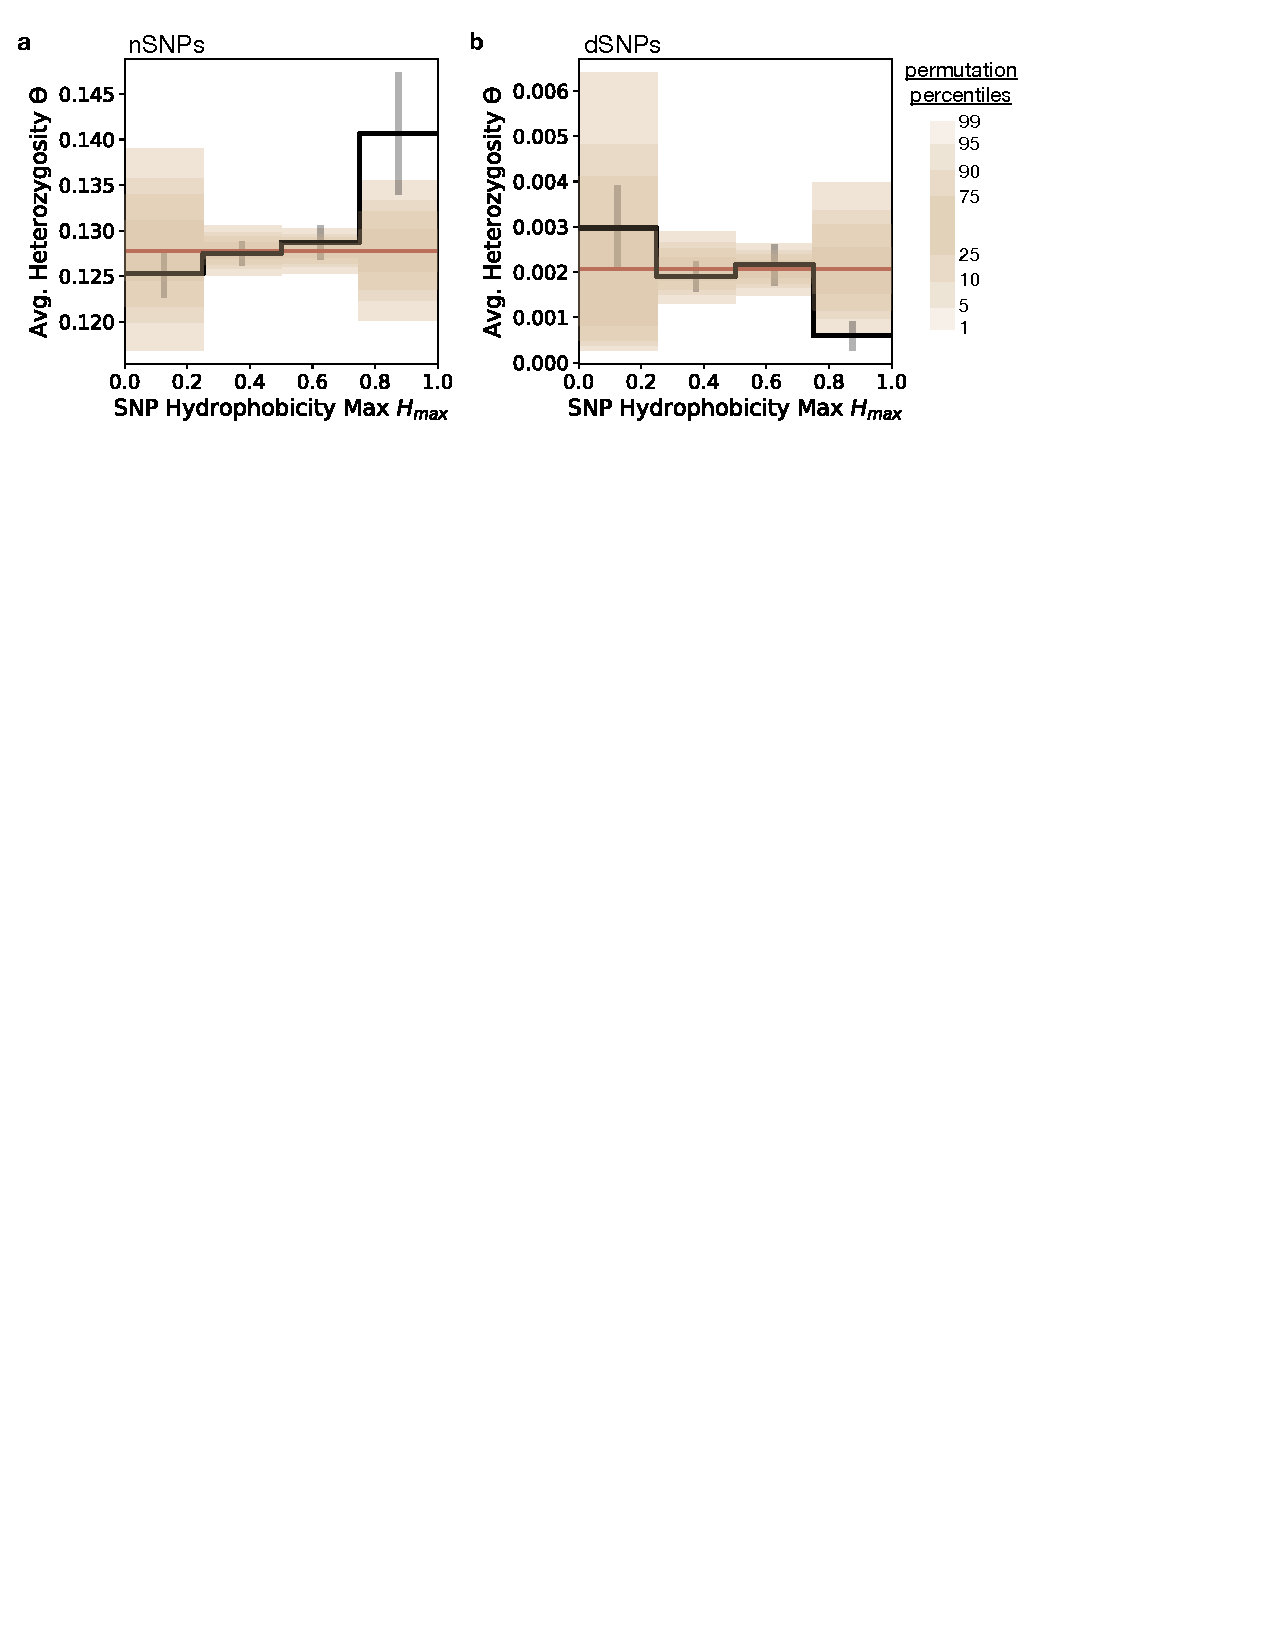
\includegraphics[width=0.6\textwidth]{fig3.pdf}
\caption{{\bf Expected heterozygosity of SNPs in Europeans as a function of blob hydrophobicity} The black line shows the average expected heterozygosity $\het$ for (a) \nSNPs and (b) \dSNPs in h-blobs, determined using unconstrained threshold blobulation ($\Lmin=4$) and binned by the resulting maximum SNP hydrophobicity $\cmax$. $\cmax$ bins have width $\Delta \cmax=0.25$ and error bars represent standard errors in the mean for that bin. Only SNPs where at least one of two alleles are in an annotated h-blob are considered. Frequencies are  from the gnomAD cohort of non-Finnish Europeans~\cite{Karczewski2021} . The horizontal brown line is the average heterozygosity for the SNPs in each panel.
%, with values (a) 0.128 and (b) 0.0021. 
The background null distribution is generated from random permutation of frequency assignment among nSNPs and among dSNPs, respectively, and is shown as brown shaded regions, with the null percentiles shown in the legend on the right.\aucomment{This figure has been updated for readability, same data as original figure} }
\label{fig:het_v_hydromax} 
\end{SCfigure*}

The results of stratifying the genetic diversity of SNPs by their surrounding maximum blob hydrophobicity is shown in Fig. \ref{fig:het_v_hydromax}. 
The population frequencies are based on non-Finnish Europeans \cite{Karczewski2021} (Dataset S5), for which the UniProt dSNP and nSNP functional annotations are expected to be reasonably accurate.
The average heterozygosity of nSNPs in low hydrophbicity domains ($\cmax\le 0.25$) is $0.125$ (Fig. ~\ref{fig:het_v_hydromax}A), while that for dSNPs is 40 times lower, 0.003 (Fig. ~\ref{fig:het_v_hydromax}B). For both nSNPs and dSNPs, the genetic diversity shows a significant departure from the neutral expectation (outside the $1^{\rm st}-99^{\rm th}$ null percentiles) for the largest $\cmax$ bin, $\cmax \geq 0.75$. For nSNPs, the heterozygosity is larger than expected ($>99^{\rm th}$ null percentile), indicative of balancing selection. In contrast, for dSNPs the heterozygosity is smaller than expected ($<1^{\rm st}$ null percentile), indicative of greater purifying selection in highly hydrophobic blobs. In other words, the disease-associated alleles in highly hydrophobic blobs appear to be more deleterious than disease-associated alleles in lower hydrophobicity blobs. 

The results here may explain the non-monotonic behavior of the dSNP-to-nSNP enrichment seen in Fig. \ref{blob_vs_window}C,D for both the moving window and blobulation calculations. The thin band of ``red'' over the bins with the highest hydrophobic threshold that still contain data indicates a depletion in the number of dSNPs relative to nSNPs. Before examining the population frequency data, it was not clear if the lack of dSNPs relative to nSNPs is due to increased selection against dSNPs, increased balancing selection for nSNPs, or a mixture of both. In this section we have shown that the heterozygosity of dSNPs decreases with higher blob hydrophobicity while the heterozygosity of nSNPs rises with blob hydrophobicity. This suggests that the depletion observed in Figs. \ref{blob_vs_window}C,D in the high hydrophobicity regions is caused by both increased selection against disease-associated alleles and increased selection for the maintenance of polymorphisms in the non disease-associated variants. 

We tested whether the trends observed in Fig. \ref{fig:het_v_hydromax} are specific to non-Finnish Europeans by performing the same analysis based on East Asian population frequencies (see {\em SI Appendix}, Fig. S1, and Dataset S5).
The East Asian frequency dataset contains an order of magnitude fewer individuals than the non-Finnish European data, $n\sim 1,500$ {\it vs} $n\sim 32,000$ individuals, which means the frequency resolution is worse than for the non-Finnish European data. Consequently, we do not observe the same level of statistical significance, but we do find the same trends as in the European cohort: for nSNPs there is increasing heterozygosity with increasing $\cmax$ and for dSNPs the heterozygosity decreases with increasing $\cmax$. The stratification of genetic diversity with blob properties appears to be a feature shared across diverse human populations.

For additional context on the proteins containing the blobs in the $\cmax\geq 0.75$ bin we use gene-ontology and pathway enrichment tests (see {\em Materials and Methods}, Dataset S6). The nSNPs found in blobs with $\cmax\geq 0.75$ are distributed across a subset of proteins ($n=635$), which we test against the background of all proteins containing nSNPs ($N=10,406$).  For the dSNPs, there are $n=179$ proteins containing the $\cmax\geq 0.75$ SNPs and a total background of $N=1,803$ proteins containing a dSNP. Both the $\cmax \geq 0.75$ nSNP and dSNP proteins are most enriched for being located in or on a membrane, as expected for proteins containing highly hydrophobic blobs. In terms of molecular function and biological process, however, the nSNPs and dSNPs differ in their enriched ontologies. The $\cmax\geq 0.75$ nSNPs are enriched for olfactory processes, chemical sensing, and signal transduction. This accords with previous observations that olfactory-related genes exhibit signs of balancing selection~\cite{Alonso2008} and/or relaxed purifying selection~\cite{Pierron2013}. This analysis has essentially re-identified this same feature of greater diversity in chemical sensing pathways, found here because the increased genetic diversity is specifically present in highly hydrophobic subdomains of those proteins. In contrast, the $\cmax\geq 0.75$ dSNPs are enriched for cation and small molecule transmembrane transport proteins. These SNPs reside in proteins enriched for critical membrane bound transporters, consistent with the signal of higher functional constraint.

\subsection*{\dSNP enrichment emerges in shorter and more weakly-hydrophobic blobs for aggregating proteins}
\aucomment{This section was reorganized to correspond with the order of the panels in Figure 4, and to emphasize the distribution shift in Panel D as a culminating result.}
Side-chain hydrophobicity plays a well-established role in diseases involving aggregating proteins~\citep{ConchilloSole2007, Fang2013, Tartaglia2008}. In order to test whether the trends observed in Fig. \ref{blob_vs_window}D are amplified in aggregating proteins, we separated aggregating proteins from the primary data set. Proteins involved in the formation of extracellular amyloid deposits or intracellular inclusions with amyloid-like characteristics are included in the ``Aggregating proteins''  subset (28 proteins, 124 nSNPs, 330 dSNPs), while all remaining proteins are labelled as ``Non-aggregating proteins''. 

First, we used whole-sequence blobulation ($\Ht=0.4, \Lmin=4$) to compare the distributions for aggregating and non-aggregating proteins across two different approaches for blob characterization. In addition to the \hydrochar{} of previously discussed analyses, blobs were also assigned \chargechar{} (Fig. ~\ref{agg_enrich}B), which is the predicted globular phase according to Das and Pappu~\citep{Das2013}. This property is calculated using the fraction of positive and negative charges in a blob, and is particularly relevant for IDPs. 
Nearly all structured proteins fall in the Class 1 (weak polyampholyte) part of the Das-Pappu phase diagram. In contrast to structured proteins, IDPs can be found in all five Das-Pappu phases, including Class 2 (Janus or boundary region), 3 (strong polyampholyte), 4 (negatively-charged strong polyelectrolyte), and 5 (positively-charged strong polyelectrolyte). 

The blob \hydrochar{} and \chargechar{} are fundamentally correlated; while blob \chargechar{} does not explicitly consider hydrophobicity, increasing the number of charged residues will reduce the average hydrophobicity of a blob. The extent of this correlation is shown in  Fig. ~\ref{agg_enrich}A, which breaks down the fraction of h- and p-blobs that fall in each Das-Pappu \chargechar. As expected, most h blobs (90\%) fall in Class 1 (weak polyampholyte), followed by 9\% in Class 2 (Janus).  The p-blobs are more evenly distributed across classes, with the highest fraction (42\%) classified as strong polyelectrolytes.  Fig. ~\ref{agg_enrich}B and ~\ref{agg_enrich}C show the SNP distributions for blobs with different \hydrochar{} and \chargechar, respectively. Since there are five charge classes and only three hydrophobicity classes, we hypothesized that in non-aggregating proteins, blob \chargechar{} would have a stronger association with disease than blob \hydrochar{}. Instead, we found that the strongest dSNP enrichment as a function of \chargechar{} (1.09 fold , \inserted{P $< 10^{-58}$} for weak polyampholyte blobs) is comparable or even slightly less than the enrichment found for \hydrochar{} (\inserted{1.15 fold, P $< 10^{-100}$} for h-blobs). 

Furthermore, the charge-based and hydrophobicity-based classification schemes yield similar trends with protein aggregation:  Fig. \ref{agg_enrich}B shows that a given \dSNP in an aggregating protein is just as likely to be found in an h-blob as if it were in a non-aggregating protein, and Fig. \ref{agg_enrich}C shows an analogous result for \dSNPs in various charge classes. However, \nSNPs in aggregating proteins are found slightly less frequently in blobs classified as h-blobs or Class 1 (globular, weak-polyampholyte) blobs than \nSNPs in non-aggregating proteins. As a result, we do observe a small increase in overall dSNP enrichment for h-blobs/weak-polyampholyte blobs of aggregating proteins relative to non-aggregating proteins.


We then used the results from unconstrained-length blobulation to further stratify the \dSNP enrichment in aggregating proteins by hydrophobicity threshold $\Ht$ and blob length. The enrichment calculations from Fig. \ref{blob_vs_window}D were partitioned between aggregating and non-aggregating proteins, and are shown in Fig. ~\ref{agg_enrich}D. The highly-enriched (blue) band is shifted toward the origin for aggregating proteins, indicating that sensitivity to mutation is found in shorter and more weakly hydrophobic blobs. \inserted{The differential enrichment values using whole-sequence blobulation in Figs. ~\ref{agg_enrich}B,C arise from collapsing the distributions in~\ref{agg_enrich}D along a single value of $\Ht$. This result suggests that lower hydrophobicity thresholds may be appropriate for predicting disease-risk in known-aggregating proteins, and underscores the importance of a multi-dimensional analysis for distinguishing between different groups of proteins.} 

\begin{SCfigure*}[\sidecaptionrelwidth][t]
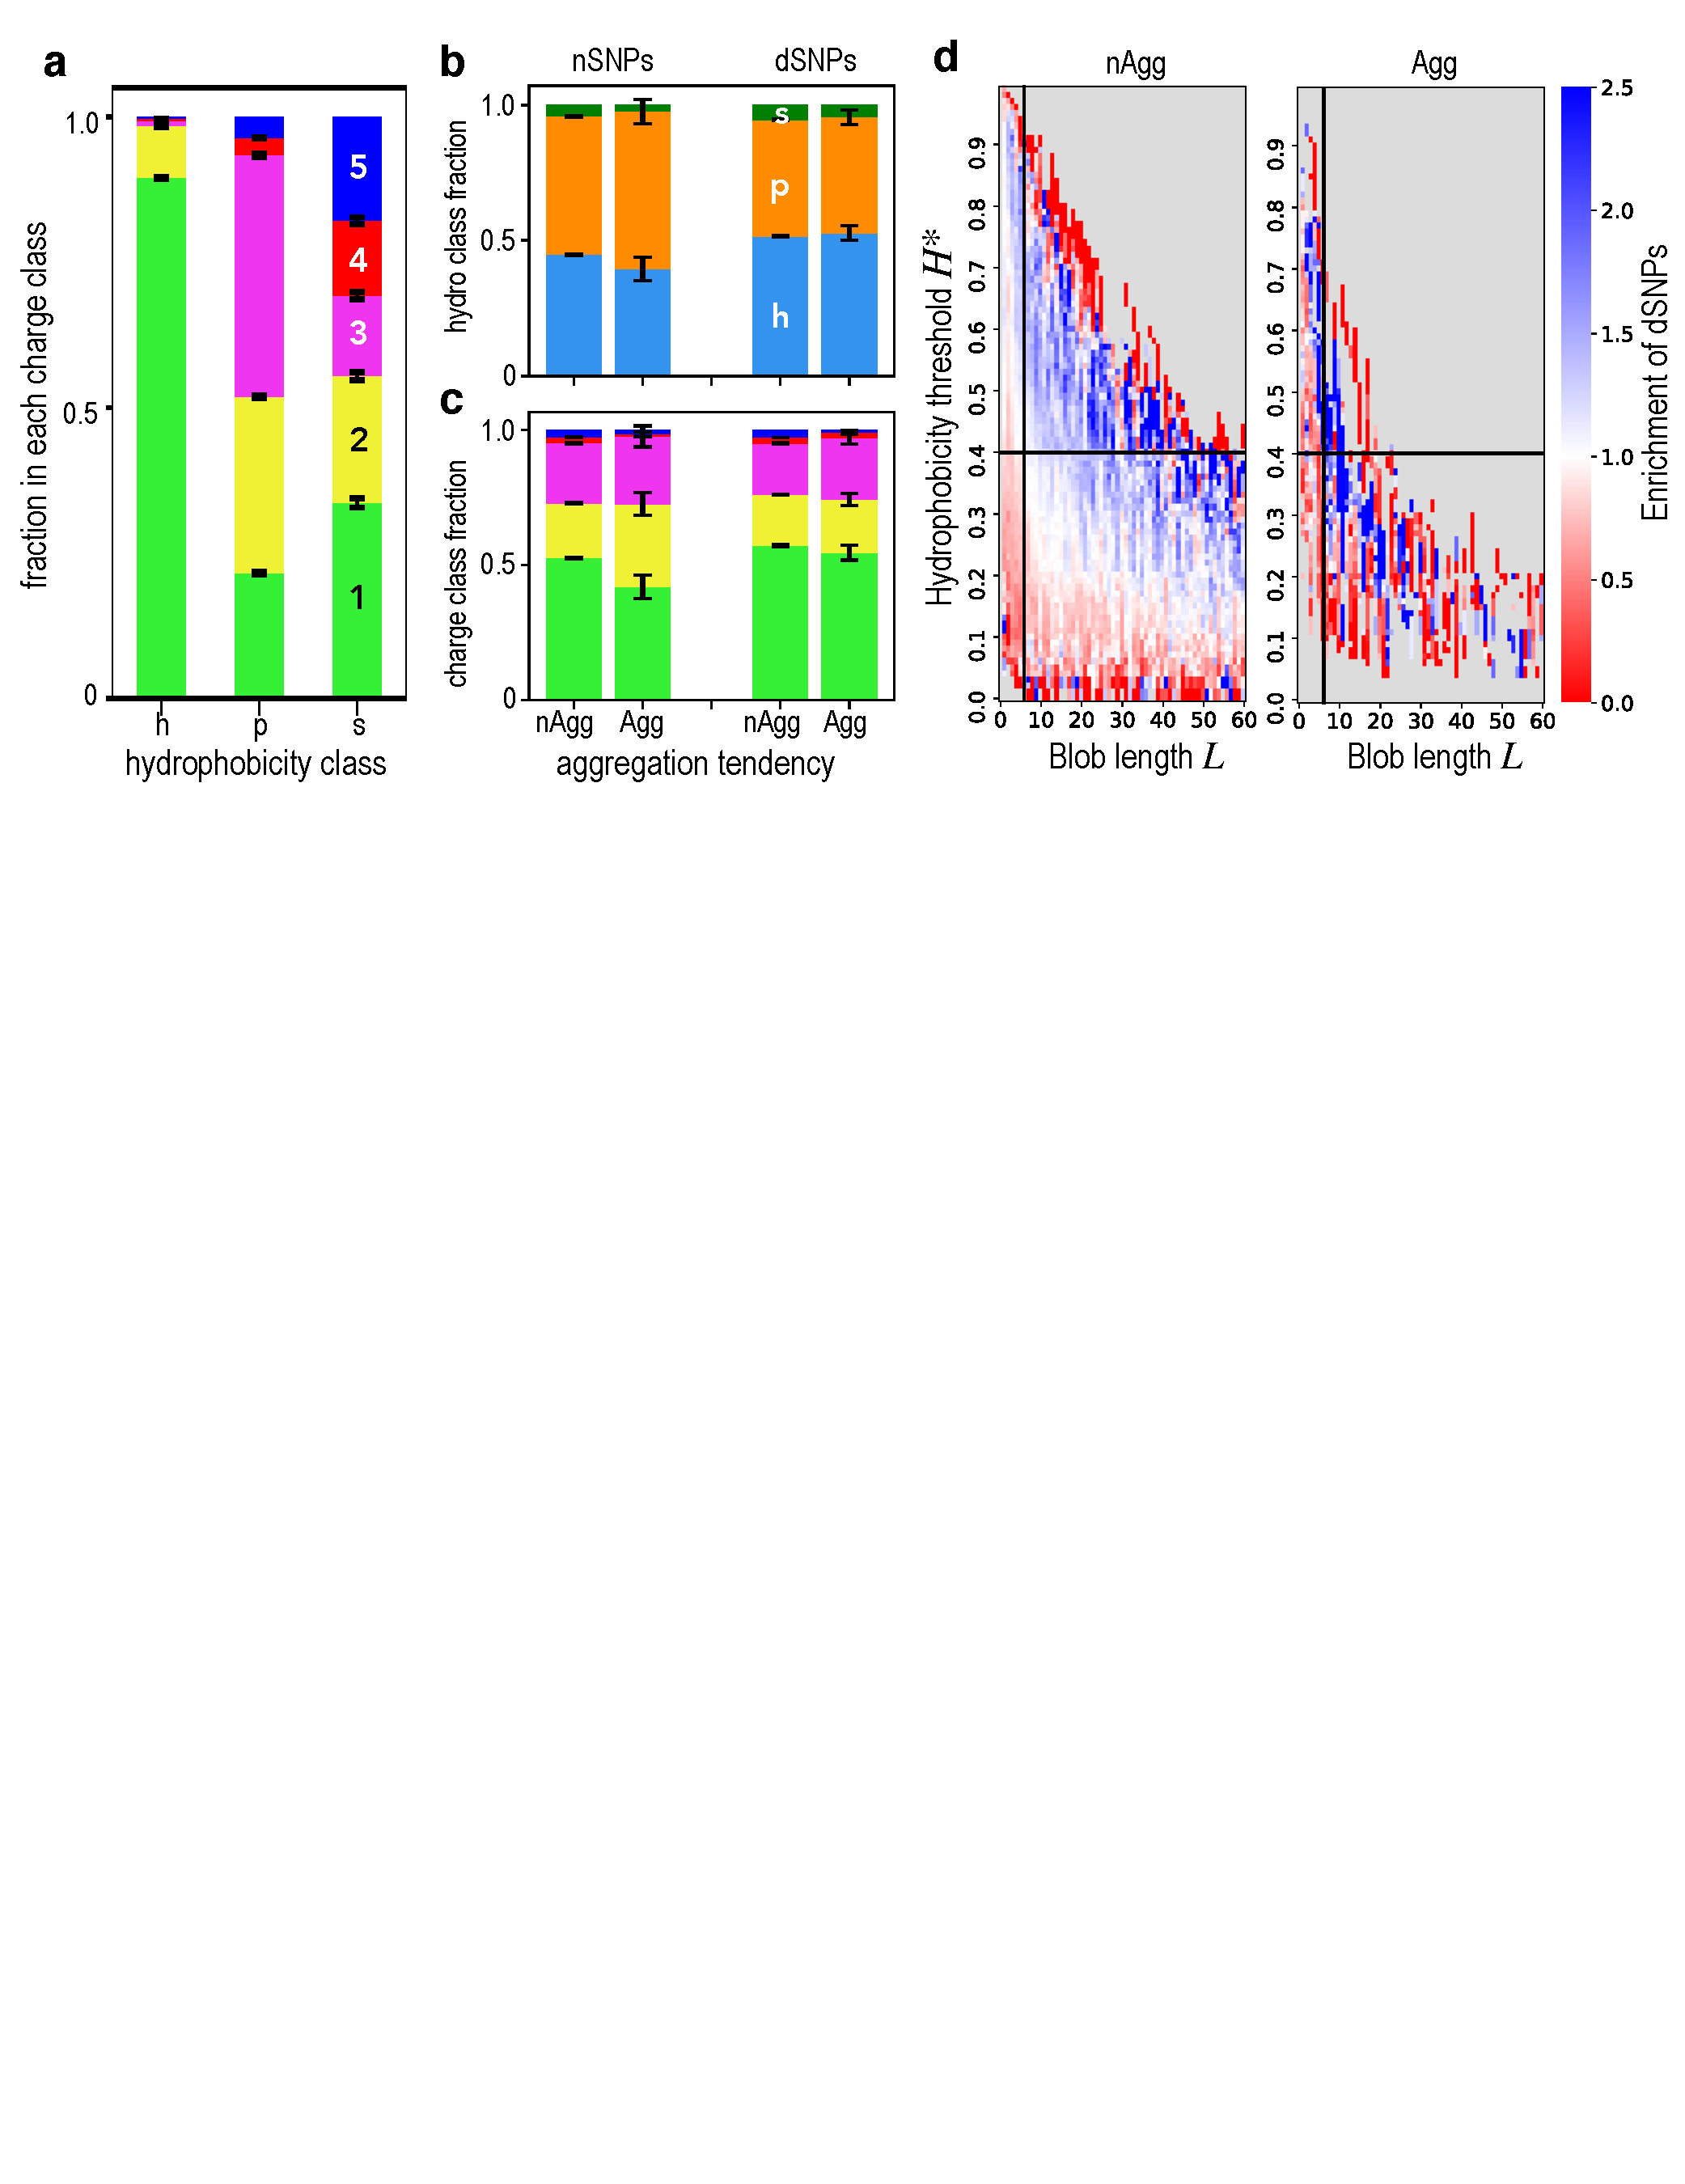
\includegraphics[width=0.7\textwidth,trim={0 0cm 0 0cm},clip]{fig4.pdf}
\caption{{\bf Blob hydrophobicity and charge properties for SNPs in aggregating proteins.} a) Distribution of \chargechar{}es (Das-Pappu~\cite{Das2013} phase) across the SNP dataset, for each blob \hydrochar. \inserted{Possible values of the blob \chargechar{} are 1 (Weak polyampholyte), 2 (Janus or boundary region), 3 (Strong polyampholyte), 4 (Negatively-charged strong polyelectrolyte), and 5 (Positively-charged strong polyelectrolyte).} b-c) Fraction of \nSNPs or \dSNPs that are found in blobs of each \hydrochar{} (b) or \chargechar{} (c) in non-aggregating (nAgg) proteins and known-aggregating (Agg) proteins. Panels (a-c) used whole sequence blobulation ($\Ht=0.4, \Lmin=4$); error bars represent one standard error for multinomial distributed data. Division of nAgg and Agg proteins is described in {\em Materials and Methods}. d) Enchriment of dSNPs binned by threshold $\Ht$ and length $L$ of the SNP-containing blob, calculated using unconstrained-length blobulation as in Fig. \ref{blob_vs_window}D, but separated by aggregation tendency. Black lines are to guide the eye. \aucomment{Panels e and f were removed to retain emphasis on the 2D distribution shift.}}
\label{agg_enrich} 
\end{SCfigure*}

\subsection*{Disease-associated SNPs are enriched for mutations that change local blob characteristics and overall protein blob topology}
\aucomment{Minor edits were made to this section for clarity.}
Whole-sequence blobulation yields a series of h-blobs, connected by p- and s-blobs, which we term the ``blobular topology''. Such a topology is analogous to the classic protein topology of secondary structure elements, although the location of edges and number of elements may be distinct. A SNP can alter the blobular topology by moving a short stretch of contiguous residues above or below the minimum blob size, either forming a new small h-blob or dissolving an existing small h-blob respectively. A SNP can also split a long h-blob by interrupting a long contiguous hydrophobic sequence, or merge two smaller h-blobs into one long h-blob by removing such an interruption. 

Here we tested whether the \dSNPs were more likely to change the topology determined by whole-sequence blobulation ($\Ht=0.4, \Lmin=4$). Figure \ref{c3_h_p_enrich}A displays the fraction of \nSNPs and \dSNPs that cause each of type of topological change. In the background case we expect to see more formation than dissolution, since the blob count decreases with length (Fig. \ref{blob_vs_window}H), and there are more blobs just below the minimum length than just above it. Figure \ref{c3_h_p_enrich}A confirms this expectation for nSNPs, and the difference between the fraction of \nSNPs and \dSNPs that form new h-blobs is not significant  (Binomial test, $P>10^{-3}$). 

%\begin{SCfigure*}[\sidecaptionrelwidth][t]
\begin{figure}
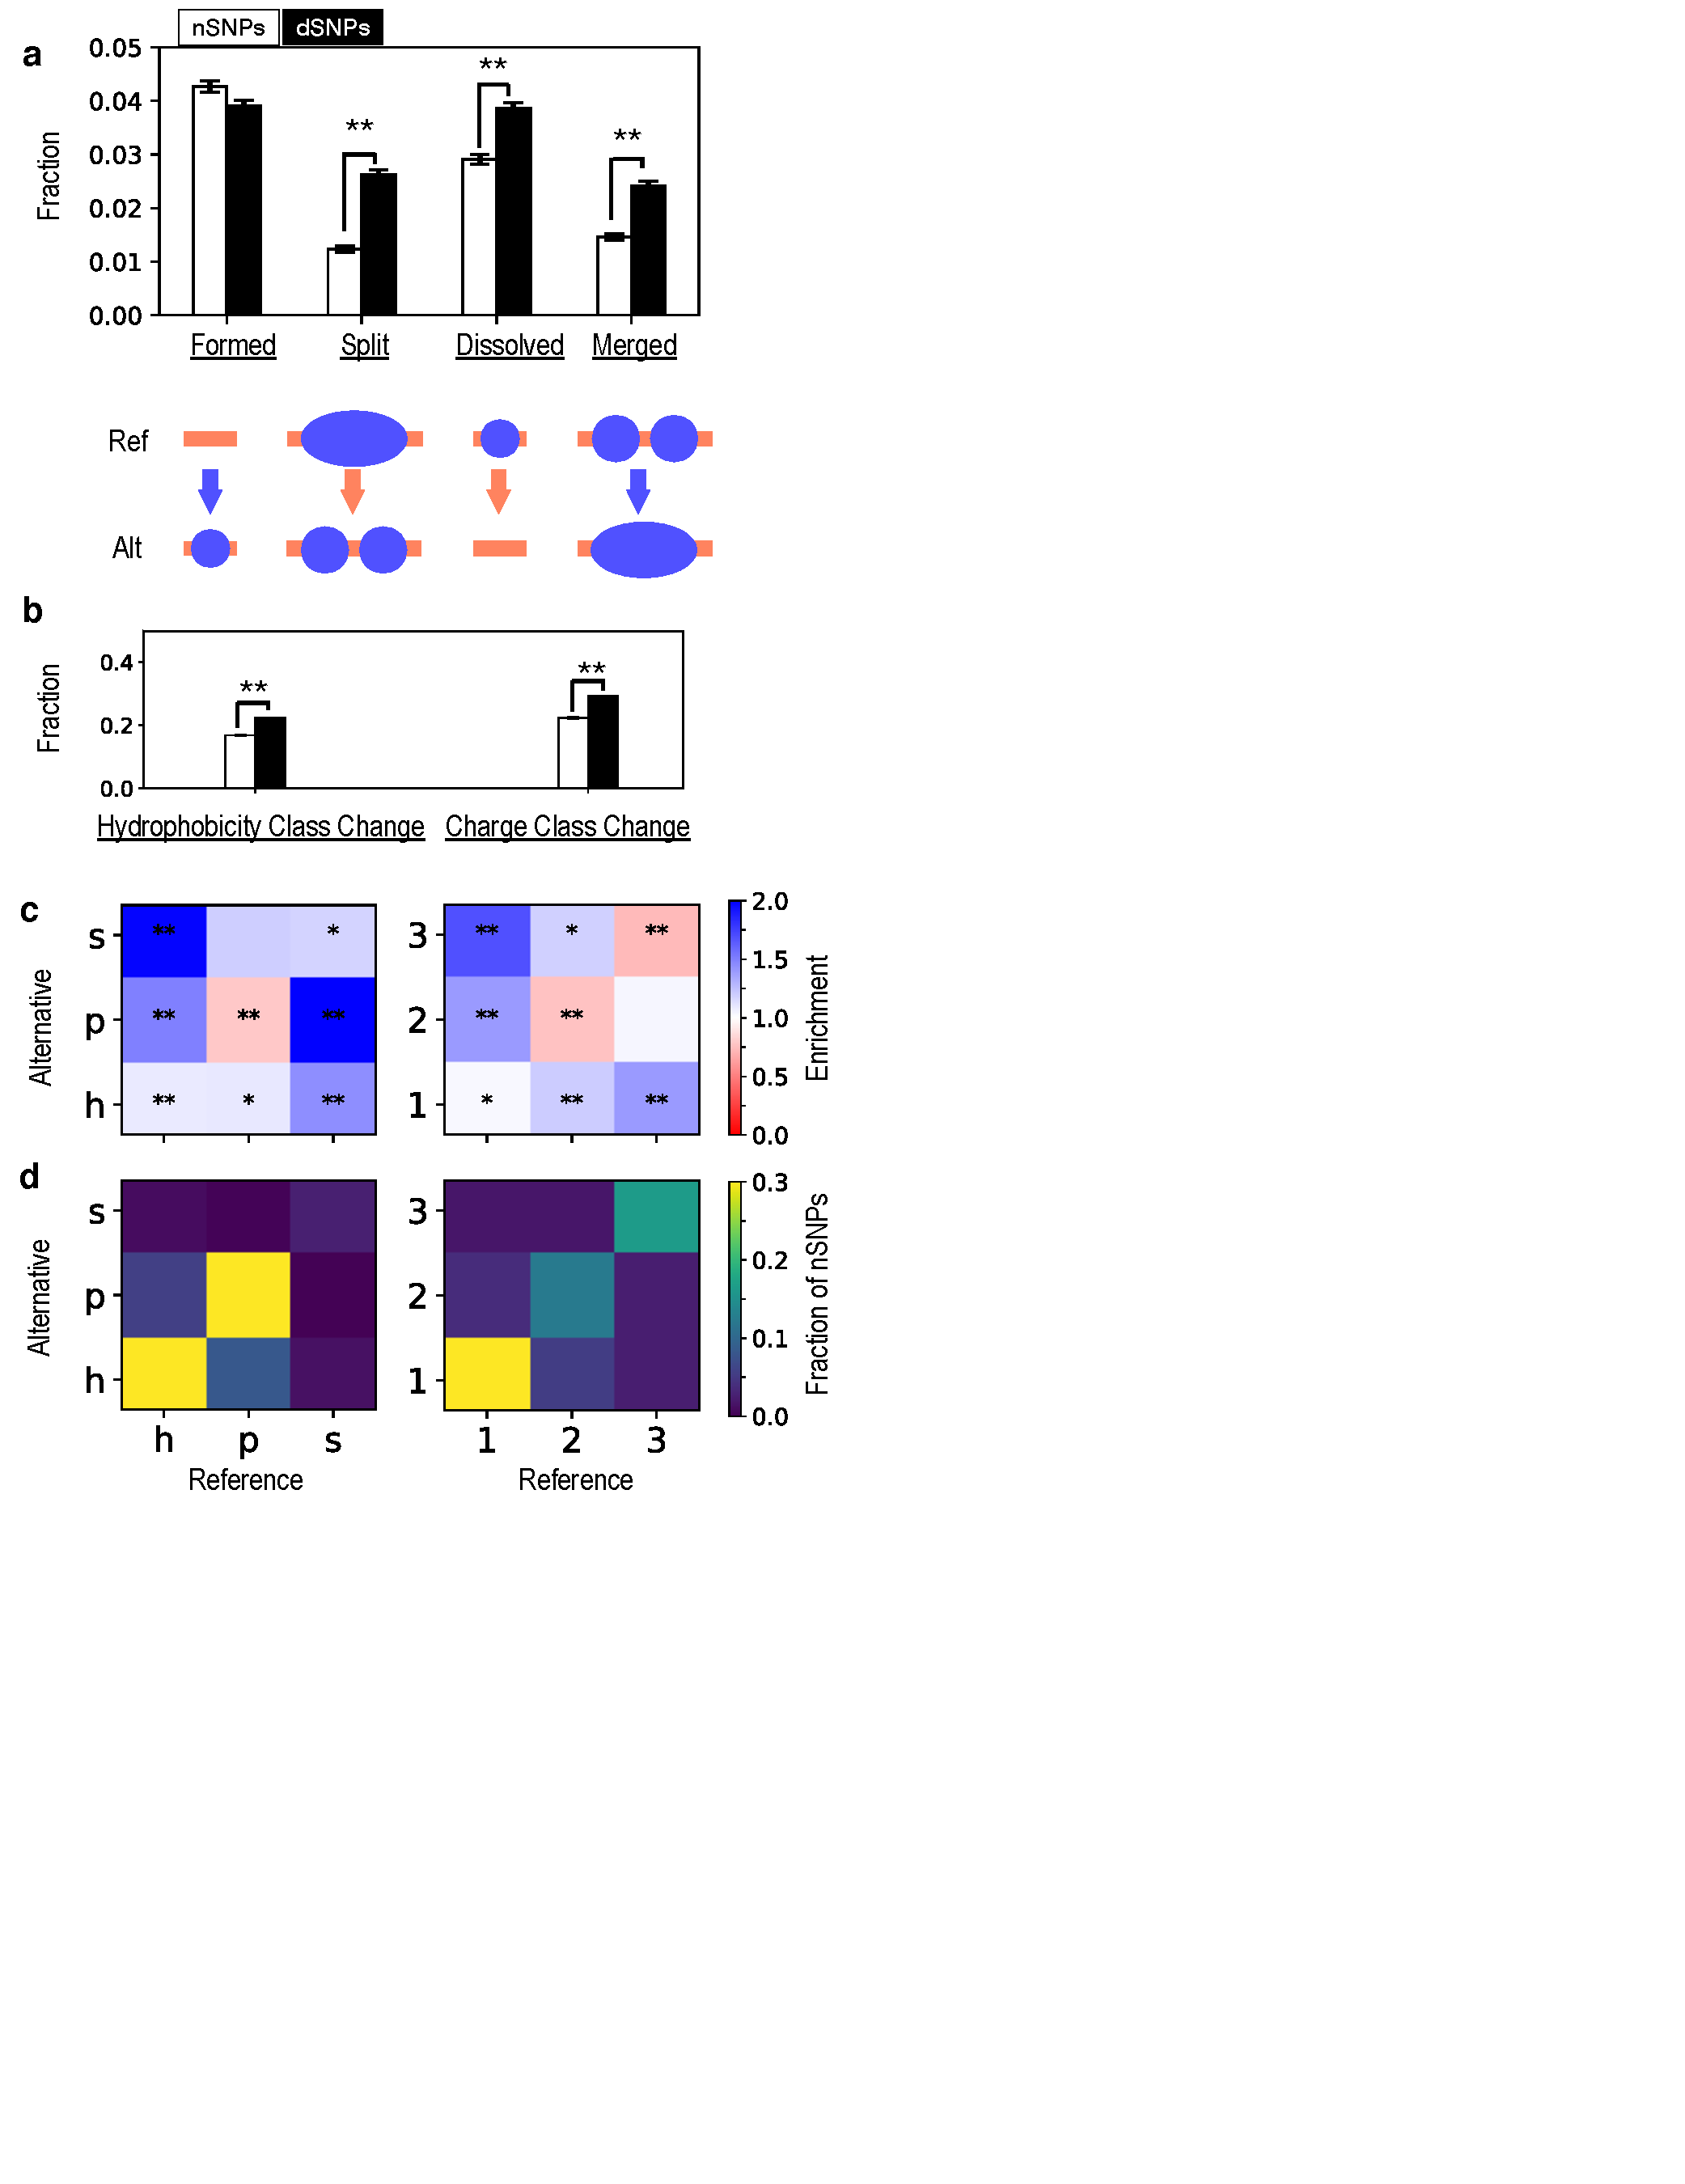
\includegraphics[width=0.5\textwidth,trim={0 0cm 0 0cm},clip]{fig5.pdf}
\caption{{\bf Distribution of SNPs that change blob properties}  a) Fraction of \nSNPs or \dSNPs that change the blobular topology by either forming or dissolving an h-blob or by splitting one h-blob or merging two h-blobs. b) Fractions of \nSNPs or \dSNPs that induce a change in \hydrochar{} or \chargechar.  c) The enrichment of \dSNPs relative to \nSNPs that induce a specific transition between the blob containing the reference allele (x-axis) and the blob containing the alternative allele (y-axis). This is shown for two blob properties, \hydrochar{} (left) and \chargechar{} (right), where the \chargechar{} categories are the same as in Fig. 4. d) The overall proportion of \nSNPs that induce each of the blobular topology transitions shown in (c).  Fewer than 1.5\% of SNPs involve charge Classes 4 or 5, and these data are not shown for readability. Significant enrichment or depletion in \dSNPs is annotated with one star ($P< 5\times 10^{-3}$) or two stars ($P< 5\times 10^{-11}$) (Binomial test). Errors bars in (a) and (b) represent one standard error in the mean.
%for multinomial (a) or binomial (b) distributed data. 
All panels use whole sequence blobulation with $\Ht=0.4$ and $\Lmin=4$.}
\label{c3_h_p_enrich}
\end{figure}
%\end{SCfigure*}

Other topological changes, however, are strongly enriched in dSNPs. As shown in Fig. \ref{c3_h_p_enrich}A, \dSNPs are significantly more likely to dissolve h-blobs (Binomial test, $P<10^{-21}$), split h-blobs (Binomial test, $P<10^{-80}$), and merge h-blobs (Binomial test, $P<10^{-36}$). The magnitude of enrichment (2.1-fold) is greatest for SNPs that split longer h-blobs into two shorter ones and is only moderately weaker for the reverse merging of two h-blobs (1.7-fold). These results are consistent with the functional sensitivity of long blobs shown in Fig. \ref{blob_vs_window}D. Regardless of overall topological changes, SNPs may change the characteristics of their local blob. Such changes may affect blob topology (as in Fig. \ref{c3_h_p_enrich}A), or simply shift blob boundaries, causing a transition in blob class at the site of the SNP. The latter case is included in the data in Fig. \ref{c3_h_p_enrich}B. We observe that about 17\% of the \nSNPs and 22\% of \dSNPs introduce a blob-\hydrochar{} change at the site of the SNP, yielding a 1.3 fold enrichment (Binomial test, $P<10^{-10}$, Fig. ~\ref{c3_h_p_enrich}B). Figure ~\ref{c3_h_p_enrich}C compares the rates of specific blob \hydrochar{} transitions. Mutations involving h $\rightarrow$ p blob transitions yield the maximum enrichment (1.5 fold, $P<10^{-10}$, Binomial test) among \dSNPs{}. In contrast, \dSNPs are only 1.1 fold enriched (Binomial test, $P<10^{-3}$) in the reverse p $\rightarrow$ h blob transition, and SNPs that remain in p-blobs for both the reference and alternative allele are depleted among disease-associated SNPs. 

Similarly, the frequency of SNP-induced changes in blob \chargechar{} is shown in Fig. ~\ref{c3_h_p_enrich}C, for transitions between blobs in Class 1 (weak polyampholyte), Class 2 (Janus), or Class 3 (strong polyampholyte). Transitions involving Classes 4 or 5 (positively or negatively-charged strong polyelectrolytes) represented fewer than 1.5 \% of the total transitions. Disease-associated SNPs are enriched for all mutations that change blob \chargechar{} and are either un-enriched or weakly depleted for mutations that do not change the local blob \chargechar. Collectively, these results are consistent with the increased mutational sensitivity of hydrophobic (and typically buried) blobs that is shown in Fig. \ref{blob_vs_window}D, while also emphasizing that mutations that change \chargechar{} are particularly likely to be causal. For instance, charge reversal of a charged residue could have particularly strong functional effects. While these effects might be amplified if the charged residue was in a weak h-blob (a possibility explained in {\em Materials and Methods}) and thus interacting with other protein residues, the charge reversal itself would not affect the blob \hydrochar{}.  

\section*{Discussion}
In the present work, we have presented the ``blobulation'' scheme for identifying interaction-rich protein regions from peptide sequence, and tested its use in detecting functional modules across the proteome. We show that hydrophobic h-blobs in solvated proteins are more likely to be buried: the h-blob SASA is 60\% that of non h-blobs. H-blobs are also nearly twice as likely to contain $\beta-$strands, supporting their proposed role as tertiary interaction-sites. We find that enrichment of disease-associated mutations in hydrophobic blobs increases with the strictness of the hydrophobic blob criteria, with greater than 4-fold enrichment for disease-association in the longest, most hydrophobic blobs. This result persists when SNPs in transmembrane domains are removed from the analysis. The range and resolution of varying enrichment is strongly damped in the {\it status quo} fixed-length moving window approach. Stratifying SNPs by their surrounding blob properties reveals genome-wide differences in blob genetic diversity, demonstrating pervasive differential selection that is tied to blob hydrophobicity. 
Combined, these observations support our hypothesis that blobulation provides a more meaningful and less noisy approach to protein segmentation than use of a fixed-length moving window.

We also find that disease-associated mutations are significantly more likely than non-disease associated mutations to change the blob topology of the sequence.  This suggests that blobulation provides a meaningful topology that can be used as a framework for sequence analysis, and which requires only the protein amino acid sequence and two parameters (minimum blob length and hydrophobicity threshold). Once blobs are identified, they can be characterized using any property of interest. As an example, in the present work, we find that disease-associated mutations are moderately enriched for mutations that cause transitions in blob~\hydrochar{} (up to 1.5 fold) and strongly enriched for mutations that cause certain transitions in blob~\chargechar{} (1.7 fold).

While we are not aware of a similar approach applied to generic proteins, hydrophobic blobs are analogous to the aggregation ``hot spots'' identified by tools such as AGGRESCAN~\citep{ConchilloSole2007}, ProA~\citep{Fang2013}, and Zyggregator~\citep{Tartaglia2008}. 
We do find that functional sensitivity in aggregating proteins follows similar trends as in non-aggregating proteins, but emerges in shorter blobs satisfying weaker hydrophobicity criteria. The difference between aggregating and generic proteins is thus quantitative, not qualitative, and demonstrates that hydrophobic interactions occur on a useful continuum. 

\inserted{We demonstrated straightforward use of blobulation in combination with another residue characterization method like the Das-Pappu \chargechar.} In this usage, blobulation only serves as the underlying segmentation approach for defining the local sequence. In principle, secondary structure prediction could be used for defining the local sequence instead. \inserted{As demonstrated by the example of ubiquitin (Fig. \ref{cartoon}E), however, secondary structure elements can cross between different faces of the protein, so secondary structure boundaries may not capture functional boundaries.} Many secondary structure prediction methods require alignment to a homologous sequence with known structure~\citep{Yang2018, Zhang2018a,Wang2017,Ma2018}, which may not be available. Yet this information is essential for secondary structure predictors to achieve their primary goal: determining \textit{which} secondary structure the segment will adopt. Predicting segmentation, however, only requires determining the segment boundaries. \inserted{Sequence-informed segmentation is a more feasible and straightforward task than structure prediction, and yet has been largely unexplored in existing sequence analysis methods.}

Improved information about the local context of a SNP, particularly those in hydrophobic blobs, could aid the identification of functional mutations. In the context of interpreting genome-wide association study results \citep{Gallagher2018}, the blob characteristics surrounding an associated variant provides metrics for fine-mapping and ranking putative causal variants. Such blob metrics could also be used as input features for predicting variant function with machine-learning algorithms, which derive their decision rules based on training datasets of annotated mutations. To this end, we provide a two-dimensional table (Dataset S4) of disease-association enrichment as a function of blob properties.

\inserted{Many of the analyses in this manuscript use the relaxed criteria for h-blobs to demonstrate that even conservative stratification yields meaningful differences. Thus, the potential applications are not limited to those residues that meet the strict criteria or have the strongest disease-association. We view the parameter sensitivity of blobulation as a methodological strength, because adjusting the two parameters allows the user to ``zoom'' in or out by tuning the number of detected edges. In our parallel development of a blobulation graphical interface (see {\em Materials and Methods} for access information), we have repeatedly observed that such tuning can bring previously-obscured sequence organization into visual focus. } 

\section*{Materials and Methods}

\subsection*{Blobulation}
\aucomment{This explanation is a major revision of the previous version.}
\inserted{The algorithm is illustrated in Fig. \ref{cartoon}A and B. As shown in Panel A, for a given peptide, every amino acid $i$ is assigned a mean hydrophobicity $H_i$, defined as the average Kyte-Dolittle~\citep{Kyte1982} hydropathy score with a window size of three residues, scaled to fit between 0 and 1. The sequence is then digitized by testing whether $H_i>\Ht$ for each amino acid; if $H_i>\Ht$ then residue $i$ is classified as hydrophobic, and if not, residue $i$ is classified as non-hydrophobic. Note that the algorithm classification is solely dependent on the Kyte-Dolittle score and the threshold $\Ht$, rather than the canonical classification of residue types. For instance, serine and threonine are not canonically hydrophobic, but typically have a hydropathy score beyond the relaxed threshold $\Ht=0.4$. Even charged residues can be classified as ``hydrophobic'' if they are surrounded by hydrophobic residues (so that $H_i>0$) and the threshold $\Ht$ is sufficiently low. }  

\inserted{After the sequence is digitized, the sequence is blobulated, as shown in Fig. \ref{cartoon}B. The algorithm first identifies all contiguous stretches of at least $\Lmin$ hydrophobic residues; these stretches are classified as ``h-blobs''. Of the remaining sub-sequences in the given peptide, those that are at least as long as $\Lmin$ are termed ``p-blobs'', while those shorter than $\Lmin$ are termed ``s-blobs''. Example effects of varying $\Ht$ and $\Lmin$ are shown in Fig. \ref{cartoon}C. The underlying software engine and a web-interface for sequence analysis with adjustable parameters are freely available as described in {\em Computational Packages}}.

\inserted{In addition to the classic ``whole-sequence'' blobulation method just described, we also use two variants that fix a reference residue $i$ and relax either of the two parameters.  ``Unconstrained length'' blobulation fixes the threshold $\Ht$ and calculates the length $L$ of the blob containing residue $i$, rather than imposing a minimum length. Similarly, ``unconstrained threshold'' blobulation calculates $\cmax$, which is the maximum possible value of $\Ht$ that would still assign residue $i$ to an h-blob that meets the fixed $\Lmin$ requirement on minimum blob length. }

\subsection*{Secondary and tertiary structural analysis}
\inserted{We used the Ensembl BioMart tool~\citep{Howe2020} to select human proteins that also had available structures in the PDB. Only one structure was chosen for each unique sequence; for those sequences with multiple available structures, we used a structure with maximum residue coverage. In total, the structural dataset contained $6,459$ proteins, each of which were blobulated with $\Lmin=4$ and $\Ht=0.4$. 
The secondary structure for each residue of a given blob type  was calculated using DSSP~\citep{Kabsch1983, Touw2015}. For the secondary structure calculations shown in Fig. \ref{cartoon}c, ``helix'' consists of alpha-helix, 3-helix and 5-helix, ``beta'' consists of isolated beta bridge and extended strand, and ``coil'' consists of all the remaining DSSP secondary structure types, including turn and bend. Transmembrane domains (identified using UniProt annotations~\citep{Bateman2021}) were removed from this dataset for the solvent-accessible surface area (SASA) calculations. For each residue, the raw SASA value was calculated using DSSP, and then divided by the residue-specific maximal accessibility~\citep{Miller1987} to determine the relative SASA.  The relative SASAs were then averaged for all residues of a given blob type. The SASA data is provided in Dataset S1, and the secondary structure data in Dataset S2.}

\subsection*{SNP datasets}
The SNP data we use is the UniProtKB literature-curated list of missense variants\\ ~(www.uniprot.org/docs/humsavar, obtained on 17-Jun-2020)~\citep{Yip2008}. Variants are annotated using the American College of Medical Genetics and Genomics/Association for Molecular Pathology (ACMG/AMP) terminology\citep{Richards2015}. dSNPs are those annotated as ``likely pathogenic or pathogenic'' ($N=30,227$), and nSNPs are those annotated as ``likely benign or benign'' ($N=39,448$). SNPs in transmembrane domains were identified using the annotations in UniProt~\citep{Bateman2021}.

\subsection*{dSNP enrichment tests}
\aucomment{This explanation is a major revision of the previous version.}
\inserted{For a given residue annotation, such as being in an h-blob, we test whether there are proportionally more dSNPs with that annotation than expected based on the proportion of nSNPs with this annotation. The enrichment we report is the ratio of the dSNP proportion over nSNP proportion. To quantify the statistical significance, we use a Binomial test on the dSNP count assuming the nSNP proportions apply. Specifically, if we observe $n$ dSNPs with a given annotation out of $N$ total dSNPs, and if the proportion of nSNPs with this annotation is $f$, then under a null model the observed dSNPs count is a Binomial experiment of $N$ ``tests'', each with independent probability of ``success'' $f$. We compute the probability of observing a count as extreme as $n$ (two-tailed) given $f$ using the python {\em scipy}~\cite{scipy2020} function scipy.stats.binom\_test($n$,$N$,$f$,alternative=``two-sided'').
%The probability of observing exactly $n$ dSNPs under the null model is $P(n)={N \choose n}f^{n}(1-f)^{N - n}$. For $n>fN$, the one-tailed statistical significance ``p-value'' of the observation is the cumulative probability $P(\geq n)$, and for $n<fN$ the one-tailed significance is $P(\leq n)$. Unless otherwise stated, we report the two-tailed p-value, given as twice the one-tailed p-value. 
}

\subsection*{Fixed-length moving windows}
 For each SNP $i$, we compute the mean hydrophobicity $\langle H \rangle_i$ within a window of length $L_w$ centered on $i$. For a given threshold $\Ht$, SNP $i$ is classified as falling in a  ``hydrophobic window of length $\Lw$'' only if $\langle H \rangle_i \geq \Ht$.  The window lengths $\Lw$ were iterated over all odd numbers between 1 and 99 (or the protein sequence length if the protein was less than 99 residues long), so that equal number of residues were included on each side of the SNP. The enrichment of dSNPs in hydrophobic windows compared to nSNPs is calculated as described in {\em dSNP enrichment tests}.

\subsection*{Population frequency data}
Frequency data is from the gnomAD v3 genomes dataset of variants for the non-Finnish European cohort: gnomad.genomes.r3.0.sites.chr*.vcf.bgz, accessed July 24, 2020, using the ``INFO/AF\_nfe\_male'' and ``INFO/AF\_nfe\_female'' tags. This cohort contains $32,299$ individuals, providing allele frequency data as low as $\sim 1/60,000 \sim 0.002 \%$. Variants with dbSNP identifications (``rsids'') were intersected with the UniProt SNP data. There are 36,025 SNPs in common (in 10,565 genes), composed of 29,653 nSNPs (in 10,143 genes) and 6,372 dSNPs (in 1,594 genes). For comparison we also analyzed the gnomAD v3 East Asian cohort, using the ``INFO/AF\_eas\_male'' and ``INFO/AF\_eas\_female'' tags. This cohort contains $1,567$ individuals. 

\subsection*{Expected heterozygosity of SNPs in h-blobs}
We apply the blobluation algorithm to every SNP $i$ to find the maximum blob hydrophobicity threshold, $\cmax$, for which at least one of the alleles remains in an h-blob with length $\geq \Lmin=4$. SNPs for which neither allele resides in an h-blob of minimum length $\Lmin$, regardless of $\Ht$, are discarded from further analysis. blobulate in increments of $\Delta H^* = 0.05$ from $\Ht=0$ to $\Ht=1$ to identify $\cmax$ with a resolution of $0.05$. We bin SNPs into four $\cmax$ bins of width $\Delta \cmax = 0.25$ and compute the mean SNP expected heterozygosity within each bin. The null distribution for each bin is computed based on $R=5,000$ random permutations of the SNP heterozygosity among the input SNP set. The preceding procedure is tabulated for nSNPs and dSNPs separately. The frequency data for the SNPs used in the analysis for Fig. ~\ref{fig:het_v_hydromax} is provided in Dataset S5.

\subsection*{Gene pathway and ontology enrichment tests}
The gene-ontology enrichment is performed using the g:Profiler web service \cite{Raudvere2019}. We use the g:GOSt functional annotation enrichment tool. Statistical p-values are adjusted for multiple-testing and ontology overlap using the g:Profiler algorithm ``g:SCS'' on a user significance threshold of 0.05. We use custom backgrounds over annotated genes only. The background used for nSNPs is all proteins containing an nSNP and the background for dSNPs is all proteins containing a dSNP. The ontology databases tested for enrichment are the g:Profiler databases as of 2019: GO Molecular Function (GO MF), GO Biological Process (GO BP), GO Cellular Component (GO CC), Kyoto Encylopedia of Genes and Genomes pathways (KEGG), Reactome pathways (REAC), WikiPathways (WP), TRANSFAC (TF), miRTarBase (MIRNA), the Human Protein Atlas (HPA), the Comprehensive Resource of Mammalian protein complexes (CORUM), and the human phenotype ontology (HP). The above results are provided in Dataset S6.

\subsection*{Identification of aggregating proteins}
There are 28 proteins within the dataset that are annotated as involved in formation of extracellular amyloid deposits or intracellular inclusions with amyloid-like characteristics: P02647, P06727, *P02655, P05067, Q99700, P61769, P01258, *P17927, P07320, P01034, *P35637, P06396, Q9NX55, P10997, P08069, *P01308, P02788, *P61626, P10636, Q08431, P01160, P04156, P11686, P37840, P00441, *Q13148, *Q15582, P02766. For analyses involving aggregation, the uniprot dataset was divided into the SNPs within these 28 proteins (``Aggregating Proteins'') and all other proteins (``non-Aggregating Proteins''). 

\subsection*{Das-Pappu charge class}
The blob \chargechar{} is a secondary blob property representing the Das-Pappu phase~\citep{Das2013}, which is determined using the fraction of positively and negatively charged residues as originally prescribed. Blobulation does not rely on \chargechar, but any blob may be assigned a \chargechar{} following blobulation.

\subsection*{Blob transitions induced by a SNP}
Whole-sequence blobulation ($\Ht=0.4,\Lmin=4$) is performed on two protein sequences, each containing either the reference or the alternate allele. The reference allele is used for all residues except $i$, even if the protein contains multiple other SNPs. Topological changes are identified via scanning the two sequences. The \hydrochar{} and \chargechar{} of the SNP-containing blob is also determined for each sequence. The proportion of dSNPs that induce a specific transition (or no transition) is tested for enrichment as described in {\em dSNP enrichment tests}, where the residue-level annotation is the specific transition caused by the SNP. 

\subsection*{Computational packages}
All computations were done in Python 3.6 using the \textit{numpy}~\cite{harris2020array}, \textit{scipy}~\cite{scipy2020}, and \textit{pandas}~\cite{pandas2020} packages. All plots are made using the Python \textit{matplotlib}~\cite{Hunter:2007} package. \inserted{Molecular images were made using VMD\cite{Humphrey1996}. As of November 2021, a webtool is available at {https://www.blobulator.branniganlab.org} .  The public repository for the blobulation software (including a script for reading output from the webtool into VMD for visualization) is available at {https://github.com/BranniganLab/blobulator}.}

\section*{Acknowledgments}

The authors acknowledge the Office of Advanced Research Computing (OARC) at Rutgers, The State University of New Jersey for providing access to the Amarel cluster and associated research computing resources that have contributed to the results reported here. MEBH is supported by NIH 1R35GM134957, R01AR076241, and ADA 1-19-VSN-02, and GB is supported by the Busch Biomedical Foundation. The authors are also grateful to Ms. Kaitlin Bassi and Mr. Connor Pitman for useful discussions and comments on the manuscript, \inserted{as well as to all other past and current members of the Blobulator development team (Ms. Kaitlin Bassi, Ms. Lindsey Riggs, Mr. Connor Pitman, Mr. Ezry Santiago-McRae, Dr. Thomas Joseph).} Finally, we are grateful to Dr. Cameron Abrams for coining the term ``blobulation'' to describe our algorithm. 

\section*{Author Contributions}
R.L. and G.B. developed the blobulation approach. R.L. wrote the blobulation software and performed enrichment analyses.  M.H. ran population-level analyses.  R.L., M.H., and G.B. contributed to study design, interpretation of results, generation of figures, and writing of the manuscript. 
 
\section*{Competing Interests} 
The authors declare no competing financial interests.
\bibliography{contig_pnas}

\end{document}
